\documentclass[a4paper,12pt,twoside]{memoir}

% Castellano
\usepackage[spanish,es-tabla]{babel}
\selectlanguage{spanish}
\usepackage[utf8]{inputenc}
\usepackage[T1]{fontenc}
\usepackage{lmodern} % Scalable font
\usepackage{microtype}
\usepackage{placeins}

\RequirePackage{booktabs}
\RequirePackage[table]{xcolor}
\RequirePackage{xtab}
\RequirePackage{multirow}

% Links
\PassOptionsToPackage{hyphens}{url}\usepackage[colorlinks]{hyperref}
\hypersetup{
	allcolors = {red}
}

% Ecuaciones
\usepackage{amsmath}

% Rutas de fichero / paquete
\newcommand{\ruta}[1]{{\sffamily #1}}

% Párrafos
\nonzeroparskip

% Huérfanas y viudas
\widowpenalty100000
\clubpenalty100000

\let\tmp\oddsidemargin
\let\oddsidemargin\evensidemargin
\let\evensidemargin\tmp
\reversemarginpar

% Imágenes

% Comando para insertar una imagen en un lugar concreto.
% Los parámetros son:
% 1 --> Ruta absoluta/relativa de la figura
% 2 --> Texto a pie de figura
% 3 --> Tamaño en tanto por uno relativo al ancho de página
\usepackage{graphicx}

\newcommand{\imagen}[3]{
	\begin{figure}[!h]
		\centering
		\includegraphics[width=#3\textwidth]{#1}
		\caption{#2}\label{fig:#1}
	\end{figure}
	\FloatBarrier
}







\graphicspath{ {./img/} }

% Capítulos
\chapterstyle{bianchi}
\newcommand{\capitulo}[2]{
	\setcounter{chapter}{#1}
	\setcounter{section}{0}
	\setcounter{figure}{0}
	\setcounter{table}{0}
	\chapter*{#2}
	\addcontentsline{toc}{chapter}{#2}
	\markboth{#2}{#2}
}

% Apéndices
\renewcommand{\appendixname}{Apéndice}
\renewcommand*\cftappendixname{\appendixname}

\newcommand{\apendice}[1]{
	%\renewcommand{\thechapter}{A}
	\chapter{#1}
}

\renewcommand*\cftappendixname{\appendixname\ }

% Formato de portada

\makeatletter
\usepackage{xcolor}
\newcommand{\tutor}[1]{\def\@tutor{#1}}
\newcommand{\tutorb}[1]{\def\@tutorb{#1}}

\newcommand{\course}[1]{\def\@course{#1}}
\definecolor{cpardoBox}{HTML}{E6E6FF}
\def\maketitle{
  \null
  \thispagestyle{empty}
  % Cabecera ----------------
\begin{center}
  \noindent
\includegraphics[width=\textwidth]{cabeceraSalud}\vspace{1.5cm}%
\end{center}
  
  % Título proyecto y escudo salud ----------------
  \begin{center}
    \begin{minipage}[c][1.5cm][c]{.20\textwidth}
        
\includegraphics[width=\textwidth]{escudoSalud.pdf}
    \end{minipage}
  \end{center}
  
  \begin{center}
    \colorbox{cpardoBox}{%
        \begin{minipage}{.8\textwidth}
          \vspace{.5cm}\Large
          \begin{center}
          \textbf{TFG del Grado en Ingeniería de la Salud}\vspace{.6cm}\\
          \textbf{\LARGE\@title{}}
          \end{center}
          \vspace{.2cm}
        \end{minipage}
    }%
  \end{center}
  
    % Datos de alumno, curso y tutores ------------------
  \begin{center}%
  {%
    \noindent\LARGE
    Presentado por \@author{}\\ 
    en Universidad de Burgos\\
    \vspace{0.5cm}
    \noindent\Large
    \@date{}\\
    \vspace{0.5cm}
    %Tutor: \@tutor{}\\ % comenta el que no corresponda
    Tutores: \@tutor{} -- \@tutorb{}\\
  }%
  \end{center}%
  \null
  \cleardoublepage
  }
\makeatother

\newcommand{\nombre}{Nuria Martínez Queralt}
\newcommand{\nombreTutor}{Daniel Urda Muñoz} 
\newcommand{\nombreTutorb}{Natalia Busto Vázquez} 
\newcommand{\dni}{71309222E} 

% Datos de portada
\title{Detección de neumonía mediante aprendizaje automático a partir de radiografías de tórax}
\author{\nombre}
\tutor{\nombreTutor}
\tutorb{\nombreTutorb}
\date{\today}


\begin{document}

\maketitle


\newpage\null\thispagestyle{empty}\newpage

%%%%%%%%%%%%%%%%%%%%%%%%%%%%%%%%%%%%%%%%%%%%%%%%%%%%%%%%%%%%%%%%%%%%%%%%%%%%%%%%%%%%%%%%
\thispagestyle{empty}


\noindent
\includegraphics[width=\textwidth]{cabeceraSalud}\vspace{1cm}

\noindent D. \nombreTutor, profesor del departamento de Digitalización, área de Ciencia de la Computación e Inteligencia Artificial.

\noindent Dña. \nombreTutorb, profesora del departamento de Ciencias de la
Salud, área de Fisiología.

\noindent Expone:

\noindent Que la alumna Dña. \nombre, con DNI \dni, ha realizado el Trabajo final de Grado en Ingeniería de la Salud titulado \textit{Detección de neumonía mediante aprendizaje automático a partir de radiografías de tórax}. 

\noindent Y que dicho trabajo ha sido realizado por el alumno bajo la dirección del que suscribe, en virtud de lo cual se autoriza su presentación y defensa.

\begin{center} %\large
En Burgos, {\large \today}
\end{center}

\vfill\vfill\vfill

% Author and supervisor
\begin{minipage}{0.45\textwidth}
\begin{flushleft} %\large
Vº. Bº. del Tutor:\\[2cm]
D. \nombreTutor
\end{flushleft}
\end{minipage}
\hfill
\begin{minipage}{0.45\textwidth}
\begin{flushleft} %\large
Vº. Bº. del Tutor:\\[2cm]
D. \nombreTutorb
\end{flushleft}
\end{minipage}
\hfill

\vfill

% para casos con solo un tutor comentar lo anterior
% y descomentar lo siguiente
%Vº. Bº. del Tutor:\\[2cm]
%D. nombre tutor


\newpage\null\thispagestyle{empty}\newpage




\frontmatter

% Abstract en castellano
\renewcommand*\abstractname{Resumen}
\begin{abstract}

La \textbf{neumonía} es una infección respiratoria aguda que afecta a las vías respiratorias y a los alvéolos. Causando que los sacos de aire, o alvéolos, en los pulmones se llenen de líquido o pus, lo que provoca su inflamación. 

Se trata de una de las principales causas de muerte tanto en niños como entre personas mayores con una tasa de mortalidad anual de 2,5 millones en los últimos años. El diagnóstico precoz es imprescindible para un correcto tratamiento.

Para su diagnóstico se emplean diversas técnicas como la resonancia magnética (RM), la radiografía de tórax (CXT por sus siglas en inglés) y la tomografía computarizada (TC). La CXT es una de las técnicas más empleadas y útiles a la hora de diagnosticar neumonía debido a la gran cantidad de información que ofrece. Aunque, también puede producir resultados confusos incluso para radiólogos especializados debido a la similitud que existe entre estas imágenes y las de otras anomalías pulmonares como el cáncer de pulmón o el exceso de líquido.

Por ello, este trabajo se enfoca en proporcionar ayuda al personal médico en el diagnóstico de neumonía a partir de la interpretación de imágenes médicas como las CXT por medio de la inteligencia artificial (IA), con el objetivo de adelantar el diagnóstico y mejorar su precisión.

\end{abstract}

\renewcommand*\abstractname{Descriptores}
\begin{abstract}
CXT, Neumonía, Redes Neuronales, Infiltrado pulmonar, Aprendizaje profundo
\end{abstract}

\clearpage

% Abstract en inglés
\renewcommand*\abstractname{Abstract}
\begin{abstract}
\textbf{Pneumonia} is an acute respiratory infection that affects the airways and alveoli. It causes the air sacs, or alveoli, in the lungs to fill with fluid or pus, causing them to become inflamed. 

It is a leading cause of death in both children and the elderly with an annual mortality rate of 2.5 million in recent years. Early diagnosis is essential for correct treatment.

Various techniques such as magnetic resonance imaging (MRI), chest X-ray (CXT) and computed tomography (CT) are used for diagnosis. CXT is one of the most widely used and useful techniques for diagnosing pneumonia because of the wealth of information it provides. However, it can also produce confusing results even for specialised radiologists due to the similarity between these images and those of other lung abnormalities such as lung cancer or excess fluid.

Therefore, this work focuses on providing assistance to medical staff in the diagnosis of pneumonia through the interpretation of medical images such as CXT images by means of artificial intelligence (AI), with the aim of advancing the diagnosis and improving its accuracy.

\end{abstract}

\renewcommand*\abstractname{Keywords}
\begin{abstract}
CXT, Pneumonia, Neural networks, Pulmonary infiltrate, Deep learning
\end{abstract}

\clearpage

% Indices
\tableofcontents

\clearpage

\listoffigures

\clearpage




\mainmatter
\capitulo{1}{Introducción}

La neumonía es una infección que afecta a uno o ambos pulmones causando que estos se llenen de líquido o pus. Entre las principales causas de la neumonía, se encuentran las infecciones bacterianas, virales y fúngicas siendo la primera de ellas la más común de todas~\cite{med24}.
Según la Organización Mundial de la Salud (OMS), la neumonía representó el 14\% de las defunciones en menores de 5 años en 2019 en todo el mundo, sobre todo en las zonas de Asia meridional y África subsahariana ~\cite{oms24}.

Un diagnóstico temprano de la neumonía es fundamental para su correcto tratamiento, pero, en ocasiones, puede ser difícil de diagnosticar debido a su similitud de síntomas con la gripe o el resfriado. Para un diagnóstico diferencial, se emplea comúnmente la CXT por ser una prueba no invasiva y relativamente económica. Aunque, también puede traer complicaciones, ya que requiere amplios conocimientos para identificar una neumonía correctamente, algo que, en muchas ocasiones ni siquiera médicos especializados son capaces de reconocer, lo que puede agravar los síntomas y empeorar su tratamiento. Esto empeora en las zonas menos desarrolladas donde es aún más complicado encontrar expertos con esas capacidades~\cite{Irfan20, kundu2021pneumonia}.

El aprendizaje profundo es una herramienta de IA que emplea redes neuronales convolucionales (CNN) para analizar grandes cantidades de datos y realizar tareas complejas de manera autónoma. Entre esas tareas, destaca la clasificación de imágenes. Esta herramienta se está empezando a emplear en el ámbito clínico, para la clasificación de imágenes médicas, por ejemplo, para identificar la presencia de neumonía en una CXT ~\cite{kundu2021pneumonia}.

Es por esto que, con este trabajo se busca dotar al personal sanitario de una herramienta basada en una red neuronal entrenada que sea capaz de identificar en una CXT de pacientes de entre 1 y 5 años una posible neumonía. Con el fin de reducir tanto los tiempos de espera como los errores garantizando una mayor seguridad en el diagnóstico y el tratamiento. 

Para ello, se han creado dos modelos distintos de CNN (AlexNet y uno de creación propia) con distintas arquitecturas e hiperparámetros (número de neuronas, tamaño de lote, etc.) hasta obtener un modelo razonablemente bueno a juzgar por diversas métricas como AUC, \textit{accuracy}, \textit{recall}, f1, etc. 

Aunque, antes de poder ser introducido en el ámbito clínico se han de realizar numerosas mejoras.

Toda la información relativa a este trabajo se encuentra en esta memoria y sus anexos correspondientes. Además existe información adicional cuya estructura está correctamente explicada en el \textit{Anexo C}.


\capitulo{2}{Objetivos}

Este trabajo tiene como propósito principal desarrollar una red neuronal capaz de identificar correctamente la presencia o ausencia de neumonía en CXT de pacientes de entre 1 y 5 años. Esto también involucra la adquisición de conocimientos acerca de la neumonía y las CXT entre otros. 

\section{Objetivos generales}

\begin{itemize}
    \item Encontrar el mejor modelo de red neuronal capaz de identificar la presencia o ausencia de neumonía en imágenes de CXT.
    \item Investigar en profundidad distintos aspectos de la neumonía tales como sus causas, síntomas, diagnósticos y tratamientos, para contextualizar la necesidad de mejora en la identificación de neumonía a partir de imágenes de radiografía de tórax.
\end{itemize}

\section{Objetivos técnicos}

\begin{itemize}
    \item Desarrollar una red neuronal convolucional (CNN) propia y compararla con la CNN de AlexNet. 
    \item Determinar la arquitectura de red neuronal óptima (en precisión y eficiencia computacional) junto con el mejor tamaño de \textit{batch size} mediante un análisis comparativo. 
    \item Comparar y determinar el número óptimo de neuronas en la capa oculta para maximizar el rendimiento del modelo.
    \item Emplear el método \textit{hold-out} para dividir los datos en entrenamiento (train), validación (val) y prueba (test). De forma que, se utilizan parte de los datos para entrenar el modelo y la otra para validarlo y probarlo. Por ende, se consigue una mejor capacidad de generalización evitando que el modelo solo trabaje bien con datos conocidos.
\end{itemize}

\section{Objetivos personales}

\begin{itemize}
    \item Profundizar en el conocimiento de la fisiología y patología del sistema respiratorio, con especial atención a la neumonía.
    \item Recordar y afianzar viejos conocimientos acerca de LaTex y GitHub.
    \item Profundizar en el conocimiento de las CXT y el análisis de sus imágenes.
    \item Afianzar conocimientos acerca de las redes neuronales.
    \item Aprender a utilizar keras, una herramienta importante en la clasificación de imágenes a partir del aprendizaje profundo.
\end{itemize}
























\capitulo{3}{Conceptos teóricos}

A continuación, se explican algunos conceptos teóricos que ayudan a comprender mejor el trabajo realizado.

\section{Conceptos teóricos básicos}

\subsection{Aprendizaje automático}
El aprendizaje automático o \textit{machine learning} es un enfoque de la IA que permite a un sistema resolver diversas tareas aprendiendo patrones a partir de los datos de entrenamiento y automatizando el proceso de construcción de modelos analíticos ~\cite{janiesch2021machine}.

\begin{figure}[h]
    \centering
    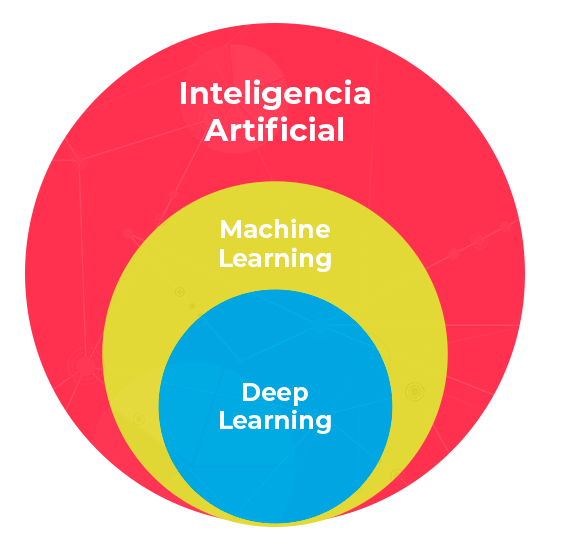
\includegraphics[width=0.40\textwidth]{img/Aprendizaje automatico.png}
    \caption{Inteligencia artifical, \textit{deep learning} y \textit{machine learning}\\  ~\cite{UniMa24}}
    \label{fig:aprendizaje_automatico}
\end{figure}
\FloatBarrier

\subsubsection{Aprendizaje profundo}
El aprendizaje profundo es un concepto de aprendizaje automático basado en redes neuronales artificiales ~\cite{janiesch2021machine} tal y como se puede apreciar en la figura \ref{fig:aprendizaje_automatico}.

En el aprendizaje profundo, la extracción de características se hace a partir de un conjunto de datos en bruto empleando múltiples capas ocultas mientras que, en el aprendizaje automático, esta extracción se realiza de forma manual, como paso previo al modelamiento\\ ~\cite{diego23}. 

Es decir, en el aprendizaje profundo las características se extraen automáticamente de los datos de entrada y se clasifican. Por otro lado, en el aprendizaje automático las características se extraen de forma manual para su clasificación o segmentación ~\cite{kundu2021pneumonia}.

El aprendizaje profundo emplea una mayor cantidad de datos y un mejor rendimiento que el aprendizaje automático\\ ~\cite{diego23}.


Entre los tipos de aprendizaje profundo se encuentran:
\begin{itemize}
    \item \textbf{Aprendizaje supervisado}: proporciona al algoritmo unos datos de entrada que, contienen las características de los datos que serán procesados y una etiqueta que los define, lo que permite, tanto entrenar un algoritmo como evaluarlo. Las CNN, las redes neuronales recurrentes o las arquitecturas tipo codificador-decodificador son ejemplos de modelos que emplean este tipo de aprendizaje\\ ~\cite{diego23}.
    \item \textbf{Aprendizaje no supervisado}: el conjunto de datos que proporciona al algoritmo está sin procesar y sin etiquetar\\ ~\cite{sindhu2020survey}. Por lo tanto, a la hora de clasificar el conjunto de datos de entrada en diversas clases, el algoritmo tendrá que identificar los patrones que caracterizan a los datos sin una referencia específica. Los algoritmos de clusterización son un ejemplo de aprendizaje no supervisado ~\cite{diego23}.
    \item \textbf{Aprendizaje por refuerzo}: aprende a realizar diversas acciones a partir de una realimentación de recompensas o penalizaciones\\ ~\cite{diego23}.
\end{itemize}

\textbf{Redes neuronales artificiales (RNA)}

Como ya se ha comentado previamente, las CNN emplean el aprendizaje profundo supervisado dentro del dominio de la IA. 

Una RNA es un paradigma de procesamiento de información para el reconocimiento de patrones y la predicción a partir de neuronas interconectadas inspiradas en el cerebro humano ~\cite{walczak2019artificial}.

El desarrollo de las RNA comenzó con la propuesta de McCulloch y Pitts (1943) de un modelo matemático de actividad neuronal en el cerebro ~\cite{walczak2019artificial}.

Los principales componentes de las redes neuronales artificiales, los cuales se pueden ver en la figura \ref{fig:w_b}, son:

\begin{figure}[h]
    \centering
    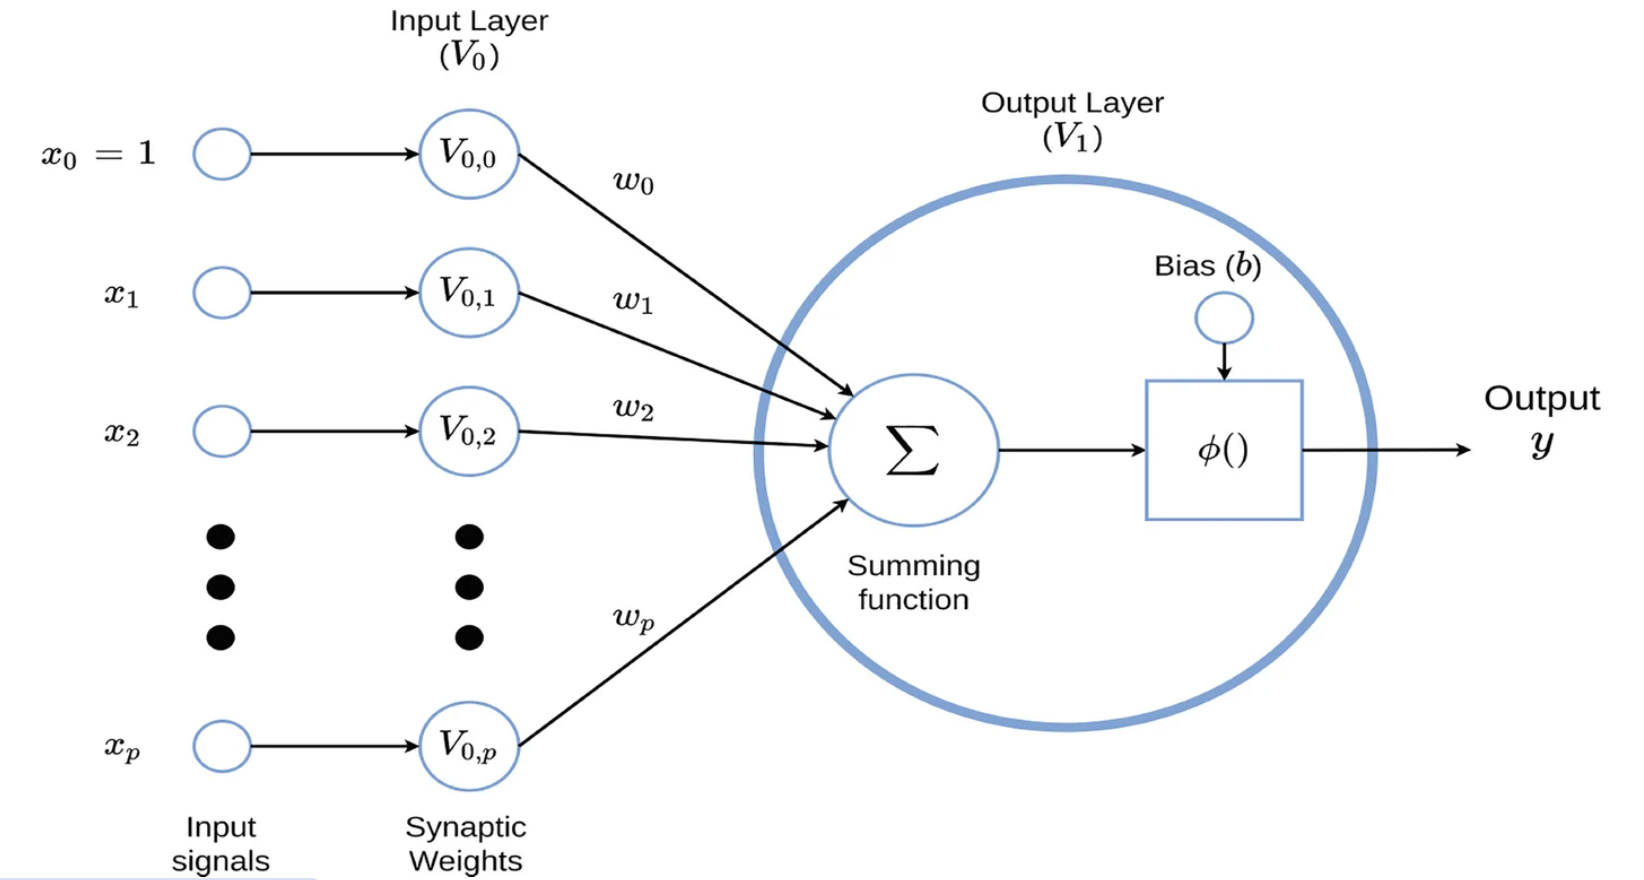
\includegraphics[width=0.99\textwidth]{img/w_b.PNG}
    \caption{Ilustración red neuronal artificial  ~\cite{montesinos2022fundamentals}}
    \label{fig:w_b}
\end{figure}
\FloatBarrier

\begin{itemize}
    \item \textbf{x1,...,xp}: es la información o señales de entrada que puede recibir la neurona tanto del sistema sensorial externo como de otras neuronas con las que tiene conexión ~\cite{montesinos2022fundamentals}.
    \item \textbf{Parámetros ``w'' (w1,...,wp)}: Es el vector de pesos sinápticos que mide la eficiencia con que la sinapsis afecta el potencial de la neurona ~\cite{montesinos2022fundamentals}. Se emplea y ajusta durante el proceso de entrenamiento para que la red neuronal pueda realizar predicciones de forma precisa ~\cite{diego23}. 
    \item \textbf{Parámetro ``b''}: Es el sesgo o umbral que se emplea para equilibrar el valor medio de las entradas con el valor medio de las salidas deseadas. Al igual que el parámetro ``w'', el parámetro ``b'' también se emplea y ajusta durante el proceso de entrenamiento para que la red neuronal pueda realizar predicciones de forma precisa~\cite{diego23}. 
\end{itemize}


\subsection{Época}
A la hora de entrenar un modelo, se realizan múltiples iteraciones sobre el conjunto de datos con un determinado tamaño de lote o \textit{batch size} (explicado a continuación), actualizando en cada iteración los parámetros ``w'' y ``b''. A estas iteraciones se las conoce como épocas\\ ~\cite{diego23}.

\subsection{\textit{Batch size}}
También denominado ``tamaño de lote'', se trata de un hiperparámetro que define el número de muestras de entrenamiento introducidas en la red para cada iteración ~\cite{link24}. Por ejemplo, si se elige un \textit{batch size}=100 y se tiene un tamaño de muestra de 2050, el algoritmo coge las muestras de 100 en 100 para entrenar la red. Es decir, toma las primeras 100 muestras y entrena la red, a continuación, coge las siguientes 100 y así sucesivamente hasta terminar con el número de muestras. En este caso, al no ser divisible el número de muestras entre 100, la solución más sencilla sería, en el último entrenamiento coger las 50 muestras restantes y entrenar la red ~\cite{stack24}.

El valor de \textit{batch size} elegido para entrenar la red tiene un impacto importante en la precisión, velocidad y estabilidad. Un \textit{batch size} mayor, indica que se procesan un mayor número de muestras en paralelo, lo que disminuye el tiempo de ejecución e implica una mayor eficiencia computacional, pero, también requiere una gran cantidad de memoria y, puede afectar a la generalización y convergencia del modelo pudiendo generar un sobreajuste, lo que puede ser un inconveniente en algunos sistemas. Por otro lado, un \textit{batch size} menor, permite actualizaciones más frecuentes de los pesos y una mejor generalización, además de un menor uso de memoria y puede evitar el sobreajuste, pero, requiere un mayor tiempo de entrenamiento, la eficiencia computacional es reducida y aumenta el ruido en las estimaciones de gradiente ~\cite{link24}. Por lo tanto, a la hora de elegir el mejor \textit{batch size}, se tiene que encontrar un equilibrio entre precisión y tiempo de entrenamiento.

Por todo esto, el \textit{batch size} óptimo varía según la red neuronal. Es importante probar diferentes valores de \textit{batch size} y comprobar cómo este afecta al rendimiento del modelo durante el entrenamiento. 

\subsection{\textit{Padding}}

\textit{Padding} es uno de los argumentos empleados tanto en la capa convolucional (Conv2D) como en la capa MaxPooling2D para realizar la convolución entre el filtro y la imagen de entrada a la hora de cear el modelo. La convolución consiste en aplicar un filtro (también denominado kernal) a una imagen para extraer características específicas ~\cite{diego23}.

Su objetivo principal es añadir pixeles alrededor de los bordes de la imagen de entrada. Los valores que se añaden son ceros (tal y como se puede apreciar en la figura \ref{fig:padding}) o los mismos valores del borde inicial de la imagen ~\cite{diego23}.

\begin{figure}[h]
    \centering
    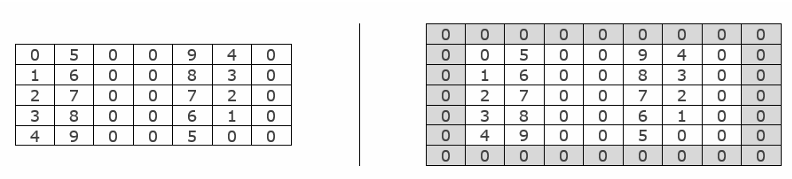
\includegraphics[width=0.99\textwidth]{img/padding.PNG}
    \caption{\textit{Padding} añadiendo ceros ~\cite{diego23}}
    \label{fig:padding}
\end{figure}
\FloatBarrier

Las opciones válidas para el argumento \textit{padding} son ``\textit{valid}'' y ``\textit{same}''. Donde ``\textit{valid}'' significa que no se aplica \textit{padding} y ``\textit{same}'' realiza el \textit{padding} de forma que, la dimensión de salida de la capa de convolución sea la misma que la de entrada ~\cite{diego23}.

\subsection{\textit{Stride}}

\textit{Stride} es otro argumento empleado tanto en la capa convolucional (Conv2D) como en la capa MaxPooling2D a la hora de crear el modelo. Se corresponde con el número de columnas y filas que se desplaza el kernal en cada operación ~\cite{diego23} tal y como se muestra en la figura \ref{fig:stride}.

\begin{figure}[h]
    \centering
    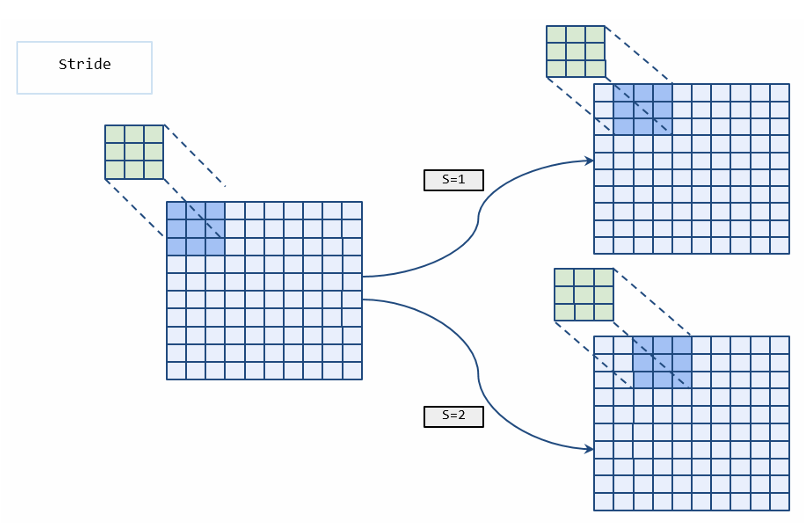
\includegraphics[width=0.99\textwidth]{img/stride.PNG}
    \caption{\textit{Stride} con valores 1 y 2 ~\cite{diego23}}
    \label{fig:stride}
\end{figure}
\FloatBarrier

Para definir \textit{stride} en keras, se debe indicar un valor entero o una tupla de dos enteros. En el caso de indicar un número entero, significa que el filtro se desplaza el mismo número para filas y columnas. Sin embargo, si se introduce una tupla, el número de filas y columnas es distinto ~\cite{diego23}.

\subsection{\textit{Overfitting}}
\textit{Overfitting} o sobreajuste, ocurre cuando el error de entrenamiento es mucho menor que el error de validación. Es decir, el clasificador tiene un error de entrenamiento muy bajo puesto que se ajusta demasiado a los datos de entrenamiento, pero, sin embargo, no es capaz de generalizar en el conjunto de validación ~\cite{diego23}.  Esto es un problema dado que, al entrenar redes neuronales, interesa que, no solo sea capaz de ajustarse correctamente a los modelos de entrenamiento, sino que también, a datos nuevos con los que se quiera trabajar. Por ello, a la hora de entrenar una red neuronal, además de los datos de entrenamiento, también se cuenta con un ``conjunto de prueba'' o ``\textit{train data}'' y uno de validación o ``\textit{validation data}''. 


\begin{figure}[h]
    \centering
    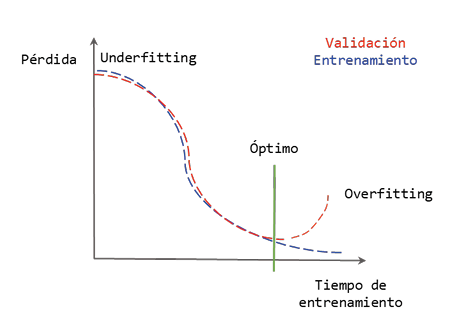
\includegraphics[width=0.70\textwidth]{img/sobreajuste.PNG}
    \caption{Ilustración del sub-ajuste (\textit{underfitting}) y sobreajuste (\textit{overfitting}) en modelos de aprendizaje automático\\ ~\cite{diego23}}
    \label{fig:sobreajuste}
\end{figure}
\FloatBarrier

Por el contrario, el \textit{underfitting} o sub-ajuste, ocurre cuando el modelo no se ajusta de forma correcta al conjunto de entrenamiento y, a su vez, tanto el error en el conjunto de entrenamiento como en el conjunto de validación es muy similar ~\cite{diego23}.

El sobreajuste está muy relacionado con el tamaño y la complejidad del modelo dado que, el modelo puede aprender el ``ruido'' o información irrelevante de los datos, lo que provoca que el modelo no pueda generalizar correctamente nuevos datos y, por tanto, no realice una buena predicción ~\cite{ibm24}.

Para reducir el sobreajuste se emplean tácticas como el aumento de los datos de entrenamiento (en número y diversidad), la reducción de la complejidad del modelo, añadir criterios de detección temprana como ``\textit{Early Stopping}'', modificar los atributos de entrada o agregar técnicas de regulación entre otras ~\cite{diego23}. 

\subsection{\textit{Early Stopping}}
Se trata de una técnica de reducción de \textit{overfitting} con la cual se agrega un criterio de detención temprana para detener el entrenamiento de forma anticipada ~\cite{diego23}.

\textit{Early Stopping} monitorea el rendimiento del conjunto de validación durante el entrenamiento y, detiene el proceso de entrenamiento cuando el rendimiento del conjunto de validación comienza a empeorar ~\cite{keras24}. Tal y como se puede apreciar en la imágen \ref{fig:sobreajuste} que aparece en la página \pageref{fig:sobreajuste} donde, la línea azul representa el conjunto de entrenamiento y la roja el conjunto de validación. La línea verde dónde pone ``óptimo'', corresponde con el punto donde \textit{Early Stopping} detendrá el entrenamiento ya que, aunque la línea del conjunto de entrenamiento continúa disminuyendo (es decir, el error o pérdida se acerca a 0), la línea del conjunto de validación comienza a ir en aumento, lo que significa que empeora.

Entre los principales argumentos incluidos a la hora de definir \textit{EarlyStopping}, se encuentra ``\textit{patience}'', el cual indica el número de épocas que tienen que pasar sin mejora para que, el entrenamiento se detenga ~\cite{keras24}. Este argumento se incluye para dejar algo de margen en el conjunto de validación en el caso de que empeore en un momento dado, pero, al cabo de un número pequeño de épocas o iteraciones vuelva a mejorar. 

\subsection{Radiografía de Rayos X}

La radiografía es una técnica de diagnóstico por imágenes que emplea rayos X para producir imágenes de las estructuras internas del cuerpo. A partir de estas imágenes, los profesionales pueden examinar y diagnosticar diversas afecciones como cáncer, roturas, problemas en los órganos internos, etc ~\cite{CliUniNa24}. Se emplea para analizar diversas parte del cuerpo pero en especial, el abdomen, tórax, huesos y dientes ~\cite{Macli24}.

Las imágenes se forman a partir del bloqueo de la radiación que producen los diferentes tejidos y estructuras del cuerpo según su densidad. Al colocar la parte del cuerpo donde se va a realizar la radiografía, entre la fuente de rayos X y la placa, se disparan los rayos X y, en la placa aparece los rayos X que han pasado según la zona. Por ejemplo, los materiales densos como huesos o metales, se observaran como zonas blancas debido a que bloquean mejor los rayos X mientras que, el aire se observara como una zona oscura ya que, no es capaz de bloquearlos ~\cite{CliUniNa24, Macli24}.

Cabe mencionar que, aunque la radiografía es de gran ayuda en algunos casos por ser un método rápido, no invasivo, de bajo coste y amplia disponibilidad, también presenta algunas limitaciones. En ocasiones, puede que en la imagen no se vea correctamente todo lo que se debería ver, como, por ejemplo, algunos tejidos blandos como tendones, músculos o ligamentos. Para estos casos se emplea la ecografía, RM o TC ~\cite{CliUniNa24}.

Los avances tecnológicos y científicos, han hecho posible la realización de radiografías con la mínima radiación posible, aumentando la seguridad del paciente a la hora de realizar este tipo de pruebas ~\cite{CliUniNa24}. 

Para más información acerca de las radiografías de rayos X consultar \textit{Anexo D}.


\subsubsection{Radiografía de tórax (CXT por sus siglas en inglés)}

La CXT es la base de las imágenes para el cribado pulmonar\\ ~\cite{gelaw15}. Con ella, se puede comprobar si existe algún problema en los pulmones, el corazón o la pared del pecho ya que, se observan los órganos y estructuras del interior del tórax\\ ~\cite{Macli24, NIH24}.

A la hora de realizar una CXT, la posición más común es la proyección postero anterior (PA), donde el paciente debe colocarse de pie en posición vertical frente a la placa de imagen. Los pies se colocan ligeramente separados para una mayor estabilidad del paciente. Las manos se colocan en las caderas y los codos hacia delante. El tórax debe estar alineado con la placa de la imagen ~\cite{gelaw15}. Esto se puede observar mejor en la figura \ref{fig:radiografia torax}. Para saber más acerca de otras vistas posibles en la CXT consultar \textit{Anexo D}.

\begin{figure}[h]
    \centering
    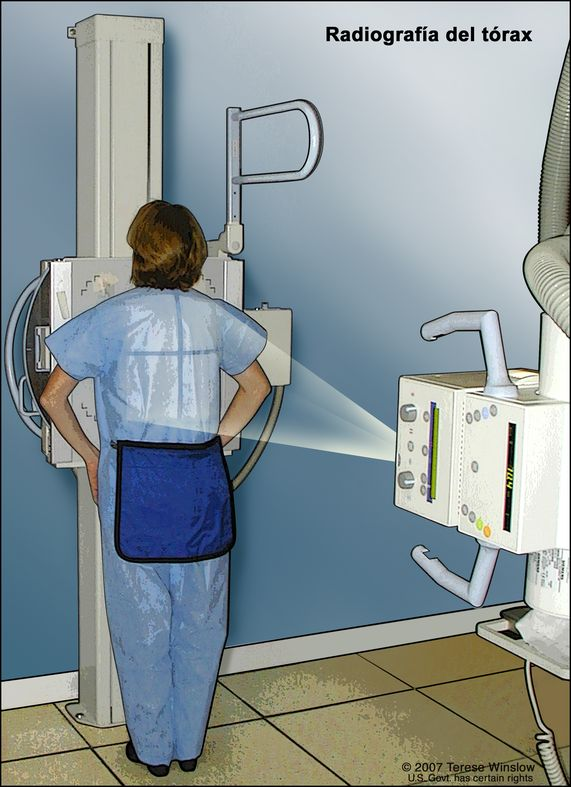
\includegraphics[width=0.44\textwidth]{img/radiografia torax.jpg}
    \caption{Ilustración CXT PA ~\cite{NIH24}}
    \label{fig:radiografia torax}
\end{figure}
\FloatBarrier

\subsection{Tomografía axial computarizada (TAC)}

El TAC es una técnica de diagnóstico por imágenes que emplea una máquina de rayos X conectada a una computadora para producir imágenes transversales del interior del cuerpo, con el fin de identificar una afección o planificar un tratamiento ~\cite{NIHTAC24}. 

El paciente se acuesta sobre una mesa (donde debe permanecer quieto) que se desplaza lentamente dentro de un escáner de rayos X en forma de anillo tal y como se aprecia en la imágen \ref{fig:TAC}. La computadora crea imágenes de la zona del cuerpo deseada en forma de cortes con las que se pueden crear modelos tridimensionales. En algunos casos, se requiere la introducción de contraste en el cuerpo por vía intravenosa o mediante la ingesta oral, para poder observar mejor algunas zonas ~\cite{MedPlusTAC24}.

Algunos riesgos de esta prueba incluyen la exposición a radiación o problemas derivados del contraste como alergias o daño a la función renal ~\cite{MedPlusTAC24}.

\begin{figure}[h]
    \centering
    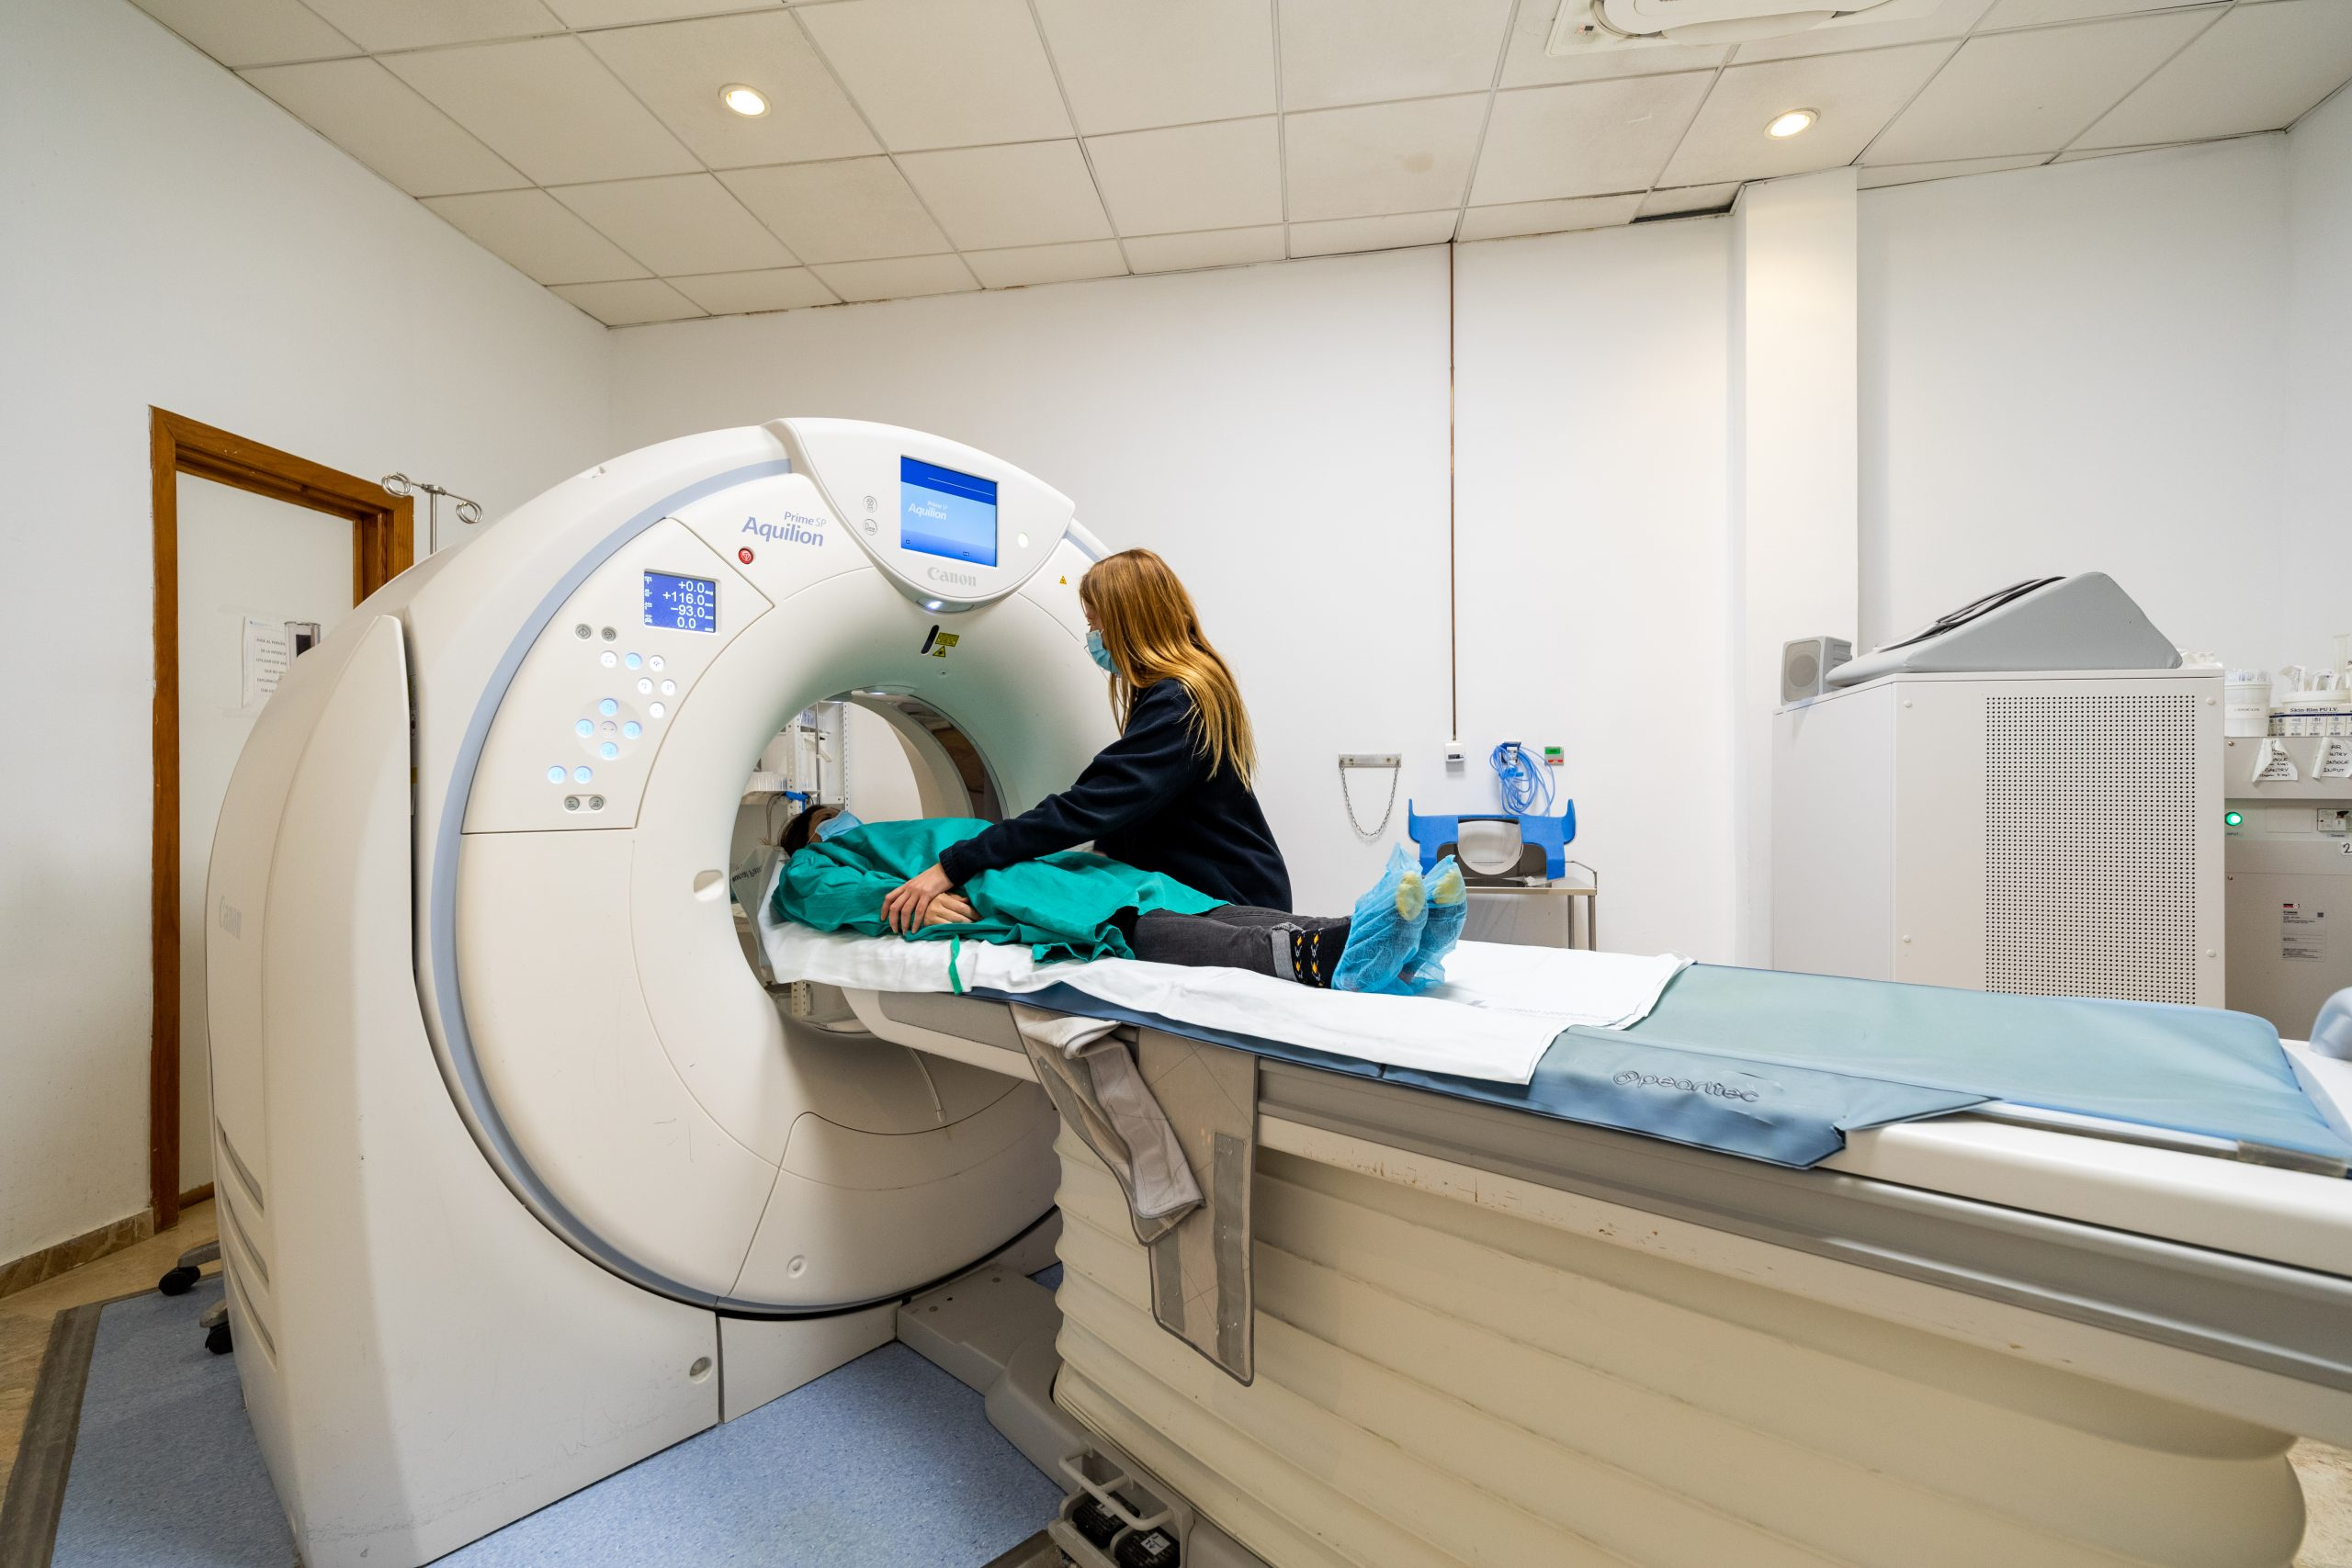
\includegraphics[width=0.70\textwidth]{img/TAC.jpg}
    \caption{Ilustración TAC ~\cite{HosPa24}}
    \label{fig:TAC}
\end{figure}
\FloatBarrier

\subsection{Opacidades blancas en la CXT}

La neumonía provoca inflamación de los alvéolos y derrame pleural, afección que consiste en una acumulación de líquido en los pulmones, lo que reduce la cantidad de oxígeno en el torrente sanguíneo provocando dificultades respiratorias ~\cite{kundu2021pneumonia}.

En una CXT, se puede diferenciar un estado saludable de un estado neumónico por anomalías como infiltrado pulmonar u opacidades blancas ya que, los pulmones sanos dejan pasar la radiación de los rayos X, por lo que se observan como zonas oscuras, a diferencia de los pulmones con algún tipo de anomalía ~\cite{gelaw15}.

Las opacidades blancas pueden ser causadas por multitud de patologías (entre ellas la neumonía) y presentan diversos patrones, algunos de ellos son:

\begin{itemize}
    \item \textbf{Consolidación}: opacidad homogénea de tamaño variable, con márgenes mal definidos e irregulares. Presenta broncograma aéreo, vías respiratorias llenas de aire vistas como líneas oscuras a través del pulmón opacificado ~\cite{gelaw15}.
    
    Su causa principal es la introducción de líquido o tejidos blandos en las vías respiratorios dificultando el paso del aire ~\cite{gelaw15}.
    
    La consolidación más típica es causada por neumonía bacteriana, aunque, también puede encontrarse en tuberculosis pulmonar\\ ~\cite{gelaw15}.
    
    \item \textbf{Colapso (atelectasias)}: opacidad y perdida de volumen que  puede afectar a los lóbulos, segmentos o subsegmentos del pulmón\\ ~\cite{gelaw15}.

    \item \textbf{Opacidades nodulares}: opacidades pequeñas y redondeadas causadas por diferentes patologías. Radiológicamente, su tamaño puede variar desde nódulos miliares (<2 mm) hasta masa pulmonar (>30 mm). Comúnmente son homogéneos (sin broncogramas aéreos) y sus bordes están bien definidos ~\cite{gelaw15, RadiopaediaPulmNodule24}.

    \item \textbf{Opacidades intersticiales}: opacidades que se observan como nódulos difusos,  sombras reticulares, reticulonodulares o líneas entrecruzadas, tal y como se puede apreciar en la figura \ref{fig:patrones_intersticial}  ~\cite{gelaw15}.

    \begin{figure}[h]
        \centering
        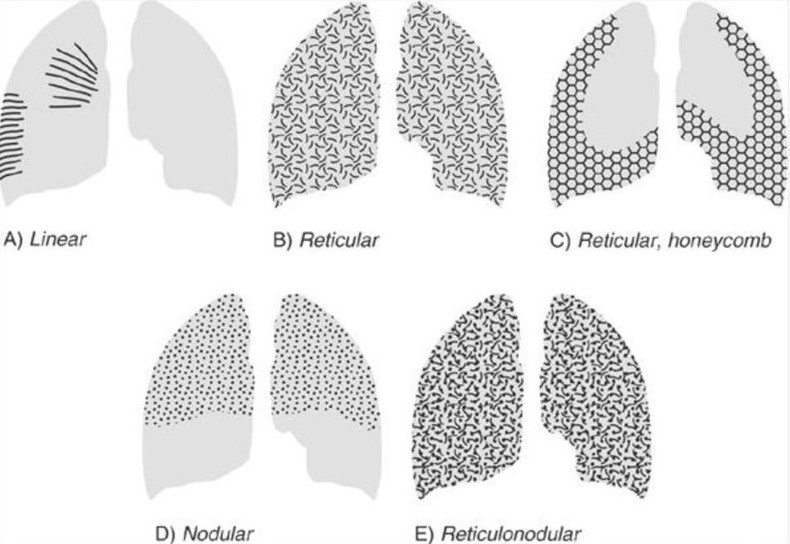
\includegraphics[width=0.99\textwidth]{img/patrones_intersticial.jpg}
        \caption{Clasificación patrón intersticial ~\cite{SlidePlayer24}}
        \label{fig:patrones_intersticial}
    \end{figure}
    \FloatBarrier
    
    Es el patrón más común de la enfermedad pulmonar intersticial difusa, la cual engloba un grupo de enfermedades pulmonares que afectan el intersticio (tejido conectivo que forma la estructura de soporte de los alvéolos) ~\cite{RadioInfo24}. Aunque, también puede verse en casos de tuberculosis en inmunocompetentes ~\cite{gelaw15}. 

    \item \textbf{Opacidades pleurales de la pared torácica}: pueden ser causadas por derrame pleural (líquido en la cavidad pleural), engrosamiento pleural (espesor de la pleura mayor de 3 mm), calcificación (proceso mediante el cual el calcio se acumula en el tejido corporal provocando que este endurezca) o por masa que surge del tejido blando ~\cite{gelaw15, MedlinePlusCalcificación24}. Se trata de un patrón típico de la tuberculosis.
    
\end{itemize}

Las características propias de la neumonía bacteriana para ser identificada  en una CXT son opacidades pulmonares focales segmentarias (es decir, bronconeumonía ) o lobares (es decir, neumonía lobar) \cite{RadiopaediaNeumoBact24}.

La bronconeumonía consiste en una inflamación peribronquiolar con posterior consolidación en el lóbulo pulmonar secundario. A nivel microscópico, la inflamación se puede ver como una congestión y dilatación extensa de los vasos sanguíneos y áreas de consolidación mal delimitadas \cite{RadiopaediaBronconeumonía24}.

La neumonía lobar está asociada con una consolidación homogénea y fibrosis o fisuras pulmonares de uno o más lóbulos de un pulmón. También presenta broncogramas aéreos \cite{RadiopaediaPulmLobar24}.

\section{Estado del arte y trabajos relacionados.}

\subsection{Prevalencia de la neumonía}

La neumonía es una infección respiratoria aguda que afecta a las vías respiratorias y a los alvéolos ~\cite{antoni2021}. 

A diferencia de otras patologías, la neumonía, no depende del grupo de edad ni de la parte del mundo ya que, presenta altas tasas de mortalidad y morbilidad en todos los grupos de edad y en todas las partes del mundo. Aunque, por un lado, tiene una mayor prevalencia en niños menores de cinco años y adultos mayores de sesenta y cinco años con enfermedades previas y, por otro lado, la prevalencia también varía según el lugar geográfico ~\cite{antoni2021}. 

En 2019, la neumonía causó más de 2,5 millones de muertes en todo el mundo, lo que la convirtió en la principal causa de mortalidad por enfermedades infecciosas por encima de la tuberculosis y el VIH ~\cite{shi2020global}. Teniendo África unas tasas de mortalidad mayores respecto a Europa y Estados Unidos (EE. UU) ~\cite{lim2022pneumonia}. Esto puede deberse a que en los países en desarrollo o subdesarrollados existe un alto nivel de contaminación, infraestructuras médicas inadecuadas y escasez de medidas higiénicas ~\cite{kundu2021pneumonia}

En EE. UU, un estudio publicado en 2015 determinó que la incidencia de neumonía adquirida en la comunidad (NAC) fue de 6,3 por cada 1000 habitantes en adultos de entre 65 y 79 años y de 16,4 por cada 1000 habitantes en adultos de más de 80 años ~\cite{jain2015community}.

En Europa, un estudio publicado en 2013 determinó que la incidencia fue de 14 por cada 1000 habitantes siendo predominante en hombres ~\cite{torres2013risk}. 

Estas diferencias entre zonas pueden deberse a los distintos sistemas sanitarios, la disminución del tabaquismo en EE. UU entre 2005 y 2016 o una vacuna neumocócica recibida en EE. UU, entre otros posibles factores. Sin embargo, la epidemiología de la neumonía manifiesta un cambio constante debido a nuevas terapias, diversas de pruebas, etc. Aunque, desde principios del siglo XXI, ha sido la causa más común de infecciones pandémicas ~\cite{jain2015community}. 

La predominancia de padecer NAC en hombres respecto a mujeres puede deberse a factores conductuales, socioeconómicos o diferencias en la anatomía ~\cite{antoni2021}. 

Además, la neumonía es la principal causa de muerte en niños menores de 5 años, con una mortalidad de 2.400 niños por día. Esta alta mortalidad puede deberse a una mayor debilidad en sus sistemas inmunológicos debido a un menor desarrollo ~\cite{saboo23}.

Las tasas de ingreso en las unidades de cuidados intensivos (UCI) difieren en distintas partes del mundo según los recursos disponibles y sus políticas de admisión. Por ejemplo, en América del Norte, más del 15\% de los pacientes hospitalizados son trasladados a la UCI, mientras que, en Europa esta cifra oscila entre el 5\% y el 10\% ~\cite{lim2022pneumonia}.

Por ello, este trabajo puede ser de gran ayuda para erradicar las distinciones entre lugares del mundo con distintas posibilidades, consiguiendo un mejor diagnóstico médico independientemente de la situación económica, social, etc. de ese país.

\subsection{Causas y tipos}

Entre las principales causas de la neumonía se encuentran las bacterias, virus respiratorios y hongos. La neumonía bacteriana, es generalmente causada por microorganismos que van desde la nasofaringe hasta el tracto respiratorio inferior ~\cite{antoni2021}.

Los patógenos se pueden transmitir entre individuos. Se trata de una infección altamente contagiosa. Además, las probabilidades de infección aumentan, en función de la existencia de algunos factores tales como, las defensas del huésped alteradas (o deficientes), la existencia de otra infección, enfermedades pulmonares previas, o un microorganismo altamente virulento ~\cite{antoni2021}.

Existen dos tipos principales de neumonía, la neumonía adquirida en la comunidad (NAC) y la adquirida en el hospital (NAH), esta última incluye la neumonía asociada a la ventilación (NAV). La NAC, a diferencia de la NAH, se contrae fuera del entorno hospitalario, en lugares como el hogar, el trabajo, el colegio, etc ~\cite{antoni2021}.

Dado que, la forma de adquirir la neumonía es distinta en NAC y NAH, las causas también son diferentes ya que, NAC es causada principalmente por \textit{Streptococcus pneumoniae}, virus respiratorios, \textit{Haemophilus influenzae} y otras bacterias como \textit{Mycoplasma pneumoniae} y \textit{Legionella pneumophila} mientras que, en el caso de NAH, las principales causan son \textit{Staphylococcus aureus}, \textit{enterobacterales}, \textit{bacilos gramnegativos no fermentadores}, y \textit{Acinetobacter spp} ~\cite{antoni2021}.

En algunos casos, la NAC puede ser causada por bacterias MRSA (resistentes a antibióticos). En estos casos el tratamiento se complica para los médicos ya que, deben identificar los factores de riesgo para estos patógenos y realizar una terapia personalizada adecuada ~\cite{antoni2021}. La NAH también puede ser causada por patógenos resistentes a medicamentos, cuya infección es más probable a medida que aumentan los días del paciente en el hospital ~\cite{lim2022pneumonia}.

Entre las características de la \textbf{neumonía bacteriana} se pueden destacar las siguientes:
\begin{itemize}
    \item Opacificación densa y bien definida en un lóbulo pulmonar.
    \item Puede existir broncograma aérea, lo que significa que, los bronquios llenos de aire son visibles dentro de una consolidación.
    \item Puede haber acumulación de líquido en el espacio pleural (derrame pleural).
\end{itemize}

Por el contrario, entre las características de la \textbf{neumonía viral}, se encuentran las siguientes:
\begin{itemize}
    \item Presentan un patrón más difuso y reticular, afectando más el intersticio pulmonar.
    \item Se pueden observar colapsos parciales del pulmón (atelectasias).
    \item Los infiltrados suelen ser bilaterales ya que, afectan a ambos pulmones de una forma más difusa.
\end{itemize}


\subsection{Síntomas y complicaciones}

Los síntomas de la neumonía incluyen dificultad para respirar, tos, disnea, dolor en el pecho, fatiga, fiebre y producción de esputo ~\cite{lim2022pneumonia}. 

A su vez, la neumonía puede estar ligada a otras complicaciones. Entre el 36\% y el 48\% de los pacientes hospitalizados por neumonía desarrollan sepsis, una disfunción orgánica potencialmente mortal causada por una respuesta desregulada del huésped a una infección ~\cite{ManualMSD24}. 

El sistema cardiovascular también se ve afectado dado que, un gran número de pacientes hospitalizados por neumonía sufre de problemas cardiovasculares tales como insuficiencias cardiacas, arritmias o síndrome coronarios agudos dentro de los siete días siguientes al diagnóstico de la neumonía ~\cite{antoni2021}. Algunos estudios también han demostrado que la neumonía aumenta en un 57\% el riesgo de padecer demencia ~\cite{shah2013bidirectional}. Cabe destacar que, la neumonía puede ser algo recurrente ya que, la tasa de reingreso de pacientes con NAC varía entre un 16,8\% y un 20,1\% ~\cite{antoni2021}.


\subsection{Factores de riesgo y prevención}

Los factores de riesgo de NAC varían en niños y adultos. En el caso de los niños, los principales factores de riesgo son la prematuridad, la desnutrición, una lactancia materna subóptima y la contaminación en las casas ~\cite{antoni2021}.
En el caso de los adultos, algunas enfermedades como la diabetes mellitus, enfermedades hepáticas y enfermedades cardiovasculares se manifiestan como los principales factores de riesgo de NAC. Otro factor de riesgo importante es la inmunocompetencia, ya que, pacientes cuyas defensas inmunitarias contra las infecciones están debilitadas presentan un mayor riesgo de NAC. Un estilo de vida poco saludable es otro factor de riesgo ya que, el tabaquismo, el alcohol o una dieta poco sana están asociados con la NAC ~\cite{antoni2021}. 

Por lo tanto, algunas maneras de prevenir la NAC implican no fumar ni beber alcohol, realizar ejercicio físico, una correcta higiene dental, evitar el contacto con niños con infecciones respiratorias y vacunarse contra la influenza y el neumococo ~\cite{lim2022pneumonia}.

En cuanto a los factores de riesgo y la mayoría de las prevenciones de la NAH, están asociadas a otros riesgos y, aún no han sido probadas. Un ejemplo de esto es, el uso de antibióticos para la descontaminación oral o digestiva que, puede ser eficaz, pero, también puede aumentar la resistencia a antibióticos. Otro ejemplo consiste en el empleo de clorhexidina para el lavado bucal, el cual puede ayudar a prevenir la NAH, aunque, estudios recientes han demostrado una mayor mortalidad en pacientes que recibieron clorhexidina ~\cite{antoni2021}.

\subsection{Tratamiento}

El lugar de recuperación de un paciente con NAC depende de su gravedad en función de una serie de factores como su frecuencia respiratoria, nivel de nitrógeno ureico en sangre, presión arterial y edad. De menor a mayor gravedad se consideran las siguientes pautas: tratamiento ambulatorio, estancia hospitalaria corta u observación cercana y hospitalización, llegando a una posible atención en la UCI en los casos más graves ~\cite{file2023community}. 

En pacientes inmunocomprometidos, los signos y síntomas usuales de una enfermedad grave pueden estar ausentes. Por ello, se requiere una vigilancia más cuidadosa y constante ~\cite{lim2022pneumonia}.

Para un correcto tratamiento de la neumonía, lo ideal es emplear biomarcadores para distinguir entre una neumonía viral o no infecciosa y una neumonía bacteriana a partir de la respuesta inmunológica del huésped. Ya que, en el caso de la primera opción no se requiere de antibiótico mientras que en la segunda sí. Pero, esto se complica en el caso de pacientes con el sistema inmunológico alterado ~\cite{lim2022pneumonia}. 

La procalcitonina es un precursor de la calcitonina (hormona peptídica involucrada en la homeostasis del calcio) sintetizado fundamentalmente en las células C del tiroides, pero también, en menor medida, en órganos como pulmones e intestino. En condiciones normales, sus niveles son bajos, pero aumentan significativamente en respuesta a infecciones bacterianas sistémicas y sepsis. La prueba de la procalcitonina se emplea para determinar si se trata de una NAC bacteriana o viral ya que, la procalcitonina es desencadenada por citocinas específicas en respuesta a bacterias. Sin embargo, a la hora de realizar la prueba de la procalcitonina también se pueden dar falsos positivos por lo que, no se deben interpretar los niveles de procalcitonina como indicadores definitivos ~\cite{file2023community}.

En el caso de la neumonía bacteriana, es preferible que el tratamiento esté dirigido específicamente al patógeno causante de la neumonía, sin embargo, normalmente, no se puede identificar este patógeno con rapidez. Por lo que, para comenzar con la terapia lo antes posible, se realiza una terapia empírica (es decir, sin conocimiento preciso de la causa o la naturaleza de la afección) que cubra los patógenos etiológicos más probables. Una vez que se obtienen los resultados de las pruebas diagnósticas (que tardan entre 48 y 72 horas), se ajusta el tratamiento para que sea específico para el patógeno identificado. Gracias a los avances en ciencia y tecnología existen nuevos métodos aprobados por la FDA (Administración de Alimentos y Medicamentos de los Estados Unidos) que proporcionan los resultados de las pruebas de diagnóstico en un plazo de 2 a 4,5 horas o incluso menos, de esta manera, se facilita un tratamiento más preciso evitando el uso innecesario o inapropiado de antibióticos ~\cite{antoni2021}.

A la hora de elegir la terapia empírica, es muy importante tener en cuenta algunos factores del paciente tales como datos epidemiológicos, enfermedades en los pulmones, corazón o hígado, diabetes, trastorno por consumo de alcohol, hospitalización reciente, lugar de adquisición de la neumonía, etc. También, hay que tener en cuenta la dosis y la vía de administración adecuadas dependiendo de la infección ~\cite{antoni2021}.  En presencia de factores de riesgo, se recomienda iniciar la terapia empírica dirigida a MRSA ~\cite{file2023community}.

En el caso de NAC grave, algunos pacientes pueden recibir corticosteroides como terapia complementaria. Esta terapia está aún en evolución, pero con evidencias positivas recientes de beneficios en pacientes con NAC grave. Se debe evitar esta terapia en pacientes con una posible gripe, influenza o neumonía por Aspergillus ~\cite{file2023community}.

Alrededor de un tercio de los pacientes con neumonía, presentan una infección con más de un patógeno. Generalmente se trata de combinaciones de patógenos bacterianos y virales ~\cite{lim2022pneumonia}.

Cabe mencionar que, aunque con un correcto tratamiento, los síntomas de la neumonía comienzan a mejorar rápidamente (dependiendo de la gravedad), no es, hasta después de 6 meses, que se logra la recuperación completa en algunos casos de NAC leve. Sin embargo, en otros casos, no se llega a conseguir una recuperación del 100\% ya que, se han observado en múltiples pacientes complicaciones cardíacas y respiratorias derivadas de la neumonía, lo que desemboca en una peor calidad de vida y un mayor grado de mortalidad a largo plazo ~\cite{antoni2021}. 

En el caso de hospitalización, el alta hospitalaria se produce cuando el paciente se encuentra clínicamente estable, puede continuar el cuidado en un entorno seguro y puede tomar medicamentos por vía oral. Se promueve el alta temprana para evitar riesgos asociados con la hospitalización, además de la reducción de costes. Pero, el paciente mantiene un seguimiento para evitar un posible reingreso en el hospital ~\cite{file2023community}.

La duración del tratamiento depende de cada caso, aunque, por lo general, suele estar entorno a un mínimo de 5 días. Este tiempo se prolonga en caso de complicaciones, pacientes con condiciones inmunocomprometidas, etc ~\cite{file2023community}.

\subsection{Diagnóstico}

El diagnóstico precoz es fundamental para poder obtener buenos resultados en el tratamiento por lo que, pruebas de diagnóstico rápidas y precisas mejoran el tratamiento ~\cite{antoni2021}. Un ejemplo de esto es que, en pacientes gravemente enfermos, iniciar el tratamiento lo antes posible, está relacionado con un menor porcentaje de mortalidad ~\cite{lim2022pneumonia}.

La CXT es el método más empleado en todo el mundo para el diagnóstico de la neumonía debido a su bajo costo y la facilidad de acceso ~\cite{li2020accuracy}. Es esencial para un correcto diagnóstico ya que, aporta información acerca del lugar concreto donde se encuentra la neumonía en el pulmón, su extensión o las características asociadas. Es de gran ayuda en la detección de opacidades pulmonares, los cuales sirven como indicadores de gravedad. Aunque, en ocasiones, es necesario complementar la CXT con la TC para una mejor detección ya que, hay infiltrados pulmonares que una CXT simple no es capaz de detectar, por ejemplo, cuando existe una neumonía recurrente, carcinoma del pulmón o empiema (pus en la capa que recubre los pulmones) ~\cite{antoni2021}.

A pesar de que la CXT sea el método más empleado en la detección de la neumonía, existen discordancias por parte de algunas personas sobre su uso ~\cite{wootton2014diagnosis}.

En el contexto comunitario, en determinadas áreas, existen desacuerdos ente realizar una CXT para confirmar un diagnóstico con sospecha de neumonía o aplicar un tratamiento empírico y, solo en caso de que este no mejore, realizar la radiografía. Esto lo hacen debido a su coste, las posibles molestias causadas al paciente, posibilidad de retraso en el diagnóstico y falta de disponibilidad inmediata para realizar una radiografía de rutina ~\cite{wootton2014diagnosis}. 

Previamente se ha comentado que, la CXT tiene un bajo coste y es no invasiva. Pero, en este caso, con el coste radiológico se refiere a la infraestructura necesaria para realizar la radiografía (que incluye equipo de rayos X y personal sanitario necesario para realizar y analizar la radiografía) ya que, ese coste puedo ser muy relevante en algunos lugares donde el acceso a la atención médica es limitado. Y, respecto a las molestias para el paciente, si bien es cierto que la CXT debería ser lo más segura posible evitando exponer al paciente todo lo que se pueda a la radiación y no es una prueba especialmente molesta, sí que existe una breve exposición a la radiación ionizante, lo que puede ser percibido como una molestia o preocupación por parte de algunas personas, especialmente si tienen que realizarse múltiples radiografías en un corto período de tiempo. Además, pueden existir molestias físicas asociadas con la posición requerida para la obtención de la imagen ~\cite{wootton2014diagnosis}.  Las diferentes posturas necesarias a la hora de realizar una CXT están correctamente explicadas en el \textit{Anexo D}.  

Hay que añadir que, al margen de las dificultades comentadas previamente por las que, en algunos lugares, en vez de realizar CXT, se basan exclusivamente en los síntomas para establecer un tratamiento, hay quien piensa que, la realización de una CXT es completamente innecesaria en algunos casos. Esta opinión se basa en las limitaciones diagnósticas de la CXT y la dificultad para interpretar dichas imágenes, especialmente por la presencia de puntos ciegos, anomalías demasiado sutiles o similitudes radiológicas con otras afecciones. Por lo que, prefieren fiarse del juicio clínico (basado en los síntomas del paciente) ~\cite{wootton2014diagnosis}.

Sin embargo, en el entorno hospitalario la CXT se realiza de manera rutinaria para confirmar el diagnóstico, y, está asociado con un beneficio clínico, lo que demuestra su importancia. También se mantiene el pensamiento de que, a pesar de los inconvenientes mencionados previamente, una CXT debería ser un requisito imprescindible para diagnosticar correctamente la neumonía (aunque, en ciertos lugares esto no puede hacerse debido a sus bajos recursos). Debido a que, se ha demostrado que un gran porcentaje de pacientes que no eran diagnosticados con neumonía basándose únicamente en sus síntomas, fueron diagnosticados con neumonías tras la realización de una CXT y, lo mismo ocurría en el caso contrario (personas sin neumonía diagnosticadas con neumonía por sus síntomas) ~\cite{wootton2014diagnosis}. Por lo que, esto no es más que un ejemplo donde se refleja la necesidad de implementar una red neuronal para la identificación de neumonía a partir de CXT que pueda ser llevada al ámbito clínico para acabar con los problemas de coste, personal y mal diagnóstico en zonas menos desarrolladas.

Otro ejemplo de esto es que, en un estudio realizado en la periferia norte de Israel, donde no existe una gran accesibilidad a las instalaciones de radiología, se ha demostrado que, la confirmación de un diagnóstico clínico de neumonía empleando CXT es fundamental ya que, en muchos casos, por falta de  accesibilidad a dichas instalaciones se diagnostica como neumonía y se trata con antibióticos a pacientes que, posteriormente con una CXT se ha demostrado que no tenían neumonía, lo que conlleva una prescripción excesiva de antibióticos y un posible desarrollo futuro de resistencia a los antibióticos ~\cite{eilat2022community}.

La ecografía pulmonar es otro método diagnóstico para la obtención de imágenes de forma no invasiva ya que, no se produce exposición a la radiación (a diferencia de la TC) y tiene un fácil empleo, aunque, puede presentar limitaciones a la hora de estudiar las capas más profundas, lo que dificulta el diagnóstico de algunas afecciones ~\cite{antoni2021}.

En el caso de pacientes hospitalizados por neumonía, es recomendable la realización de una serie de pruebas de laboratorio para un correcto diagnóstico e identificación de patógenos. Entre estas pruebas se encuentran muestras de esputo (o flema) para detectar bacterias o gérmenes que puedan causar una infección pulmonar, muestras de sangre, muestras respiratorias distales como BAL (lavado bronquio alveolar) o PCR viral en hisopos faríngeos. Esta última, se realizó sobre todo en la pandemia COVID-19 para la detección de SARS-COV-2 ~\cite{antoni2021}. En atención primaria, es poco común la realización este tipo de pruebas debido a la limitada disponibilidad de laboratorios y los tiempos prolongados para la obtención de resultados ~\cite{lim2022pneumonia}.

Algo muy importante a tener en cuenta es que, no siempre se realiza un correcto diagnóstico de la neumonía debido a su similitud tanto a nivel de características radiográficas como a nivel de sintomatología con otras afecciones pulmonares ~\cite{lim2022pneumonia}.

\subsection{Implicación del \textit{deep learning} en el diagnóstico de neumonía}

Como ya se ha comentado previamente, las radiografías de tórax proporcionan una gran cantidad de información para el diagnóstico de la neumonía, aunque, en muchas ocasiones, identificarla se vuelve muy difícil incluso para radiólogos experimentados debido a las semejanzas radiográficas que esta afección puede tener con otras afecciones como cáncer de pulmón o acumulación de líquido ~\cite{li2020accuracy}. Otros factores como la profundidad de la inspiración o la posición del paciente también dificultan la interpretación de dichas imágenes ~\cite{jaiswal2019identifying}. Por ello, el diagnóstico de la neumonía a partir de una CXT por el método tradicional, es decir, mediante la identificación de la neumonía por parte del médico a partir de la imagen, no es preciso e implica tiempo. Esto, puede derivar en un mal diagnóstico o en el retraso del tratamiento, lo que implica un empeoramiento del estado del paciente y un aumento de las tasas de morbilidad y mortalidad ~\cite{li2020accuracy}.

Por eso, a partir de los avances científicos y tecnológicos de los últimos años se ha propuesto ayudar a los médicos en la interpretación de esas imágenes con sistemas de detección asistida por computadora (CAD) basados en IA ~\cite{li2020accuracy}.

El aprendizaje profundo o DL (por sus siglas en inglés), tiene un alto potencial en el análisis de imágenes médicas gracias a su capacidad para reemplazar el proceso manual de identificación y clasificación de características en imágenes de radiografías de tórax. Su éxito, se debe principalmente a la capacidad de las redes neuronales para aprender conceptos complejos a partir de datos nuevos en un proceso de aprendizaje. Además de la detección de neumonía a partir de la CXT, el DL ha realizado avances también en el análisis de imágenes para otras afecciones como retinopatía diabética, arritmias y cáncer ~\cite{li2020accuracy}.

Se han llevado a cabo diversos algoritmos por parte de los investigadores para el análisis de las imágenes de rayos X ~\cite{jaiswal2019identifying}. Sin embargo, aún se tienen que realizar numerosos avances antes de poder incorporar el DL en el entorno clínico. Esto incluye, la precisión de los algoritmos, el correcto ajuste de los hiperparámetros, como el tamaño del lote, el número de épocas, la tasa de aprendizaje y el número de capas en las redes neuronales. Además, la cantidad y calidad del conjunto de datos juega un papel crucial. Otros aspectos importantes incluyen, el tiempo de cálculo y la tasa de error. Solo cuando se mejoren estos aspectos en su totalidad, se podrá considerar la viabilidad de llevar estos algoritmos al ámbito clínico ~\cite{jaiswal2019identifying, sharma2024systematic}.

Uno de los grandes problemas a los que se han enfrentado los investigadores es la cantidad de datos limitada ya que, al trabajar con modelos previamente entrenados, se necesitan grandes cantidades de datos además de hiperparámetros configurados correctamente para obtener los mejores resultados. Trabajar con un gran número de imágenes etiquetadas es fundamental para una correcta clasificación y predicción. Se han aplicado algunos métodos para el aumento de datos como voltear, rotar, recortar, escalar, trasladar y deformar elásticamente las imágenes para así, obtener un mayor número de imágenes ~\cite{sharma2024systematic}.

Para concluir, se puede afirmar que, existe una gran necesidad de investigación y un gran potencial de mejora en el ámbito de detección de neumonía a partir de técnicas de aprendizaje profundo ~\cite{sharma2024systematic}.




\capitulo{4}{Metodología}

\section{Descripción de los datos.}

En este trabajo, se emplean imágenes médicas de CXT frontal obtenidas a partir de un conjunto de datos público, algunas de ellas con neumonía y otras sin \footnote{\url{https://www.kaggle.com/datasets/paultimothymooney/chest-xray-pneumonia}}. Previamente a ser subidas a la plataforma correspondiente, todas las imágenes fueron examinadas minuciosamente de modo que, en primer lugar, todas aquellas imágenes que no tenían la calidad suficiente fueron descartadas. Después, dos médicos especializados evaluaron los diagnósticos de las imágenes asegurando que, estaban correctamente distribuidas en normal y neumonía y, por último, un tercer médico revisó la evaluación para evitar errores. Estas imágenes pertenecen a pacientes de entre 1 y 5 años. Se trata de imágenes con un formato .jpeg ~\cite{kaggle24}.

Para más información acerca de los datos consultar \textit{Anexo D}.
 
\section{Técnicas y herramientas.}

\subsection{Bibliotecas y herramientas empleadas}

\subsubsection{Anaconda}

Anaconda es una distribución de \textit{software} libre y comercial de lenguajes de programación Python y R, usada para la ciencia de datos y el aprendizaje automático ~\cite{wikianaconda24}. Permite la creación y gestión de entornos virtuales aislados, lo que ayuda a evitar conflictos entre diferentes versiones de paquetes. Se encuentra disponible para Windows, macOS y Linux, lo que la hace accesible a una amplia gama de usuarios ~\cite{anaconda24}.

\subsubsection{Python}

Python es un lenguaje de programación de alto nivel. Cuenta con un sistema de programación orientado a objetos ~\cite{Pyth24}. 

Entre sus beneficios, se puede destacar su eficiencia y su facilidad de uso gracias a una sintaxis clara y legible. Además, el \textit{software} es gratuito y se integra correctamente en todos los tipos de sistemas ~\cite{aws24}.

Para la realización de tareas, cuenta con una gran cantidad de bibliotecas, las cuales son de gran ayuda. Entre ellas se encuentra la biblioteca keras, la cual se emplea en este trabajo.

\subsubsection{Keras}

Keras es una biblioteca de redes neuronales profundas de código abierto escrita en Python ~\cite{wikikeras24}. Su objetivo es entrenar y compilar modelos de aprendizaje profundo.

Keras está integrada con TensorFlow, ya que es la API de alto nivel de esta plataforma por lo que, tiene acceso a todas las capacidades de esta multiplataforma ~\cite{TenFloKeras24}.

En este proyecto, se emplea esta herramienta para entrenar una arquitectura de aprendizaje automático basada en redes neuronales de forma rápida y eficiente. Estas redes determinarán la posible existencia de neumonía al realizar una radiografía.

\subsubsection{Tensorflow}

TensorFlow es una plataforma integral para el aprendizaje automático ~\cite{TenFlobasic24}.  Facilita la creación de modelos de aprendizaje automático de una forma sencilla ~\cite{TenFloint24}.

Esta biblioteca de código abierto permite el cálculo numérico basado en matrices multidimensionales. Además, es compatible con la diferenciación automática y la construcción, capacitación y exportación de modelos. Emplea la Unidad de Procesamiento Gráfico (GPU) para la realización del procesamiento distribuido, de forma que, múltiples computadoras o nodos trabajan simultáneamente para la realización de una tarea concreta o, de un conjunto de tareas ~\cite{TenFlobasic24}.

\subsubsection{LaTeX}

LaTeX es un editor de texto en línea, por lo que no requiere de ninguna instalación ni actualización de versiones. Cuenta con cientos de plantillas para comenzar a trabajar ~\cite{Over24}. Está orientado a la creación de documentos con una alta calidad topográfica ~\cite{CompHo24}.

Emplea un programa llamado motor TeX para el proceso de maquetación que se encarga de realizar de forma automática todo el aspecto visual del documento ~\cite{CompHo24}.

En este proyecto se ha empleado esta herramienta para la redacción de la memoria y los anexos.

\subsubsection{Kaggle}

Kaggle es una comunidad en línea de profesionales del aprendizaje automático y científicos de datos ~\cite{wikikaggle24}.

Es una plataforma que se emplea para buscar o publicar conjuntos de datos, resolver desafíos de ciencias de datos o emplear \textit{notebooks} con GPU integrado para no tener que emplear el ordenador local ~\cite{MaselData24}.

En este trabajo, se ha empleado esta plataforma para la obtención de las imágenes de CXT con y sin neumonía.

\subsubsection{GitHub y GitHub Desktop}

GitHub es una plataforma basada en la nube que cuenta con un sistema de control de versiones (VCS) llamado Git. Permite a los desarrolladores gestionar sus proyectos, realizar un seguimiento de los cambios en el código, colaborar con otros programadores y depositar sus repositorios de código ~\cite{HosTu24}. 

En este proyecto se ha empleado esta herramienta para la planificación de las distintas tareas realizadas, agrupando estas tareas en hitos (\textit{milestones}) y añadiéndoles etiquetas (\textit{labels}) para describirlas. Además, mediante ``GitHub Desktop'', una aplicación de escritorio gratuita, se ha clonado el repositorio del Trabajo de Fin de de Grado (TFG) de GitHub para sincronizar el código realizado en Python con las tareas estipuladas en ese repositorio.

\subsubsection{Scikit-learn}

Scikit-learn es una biblioteca de aprendizaje automático de código abierto para el lenguaje de programación Python ~\cite{wikisclearn24}.

Se trata de una herramienta simple y eficiente para el análisis predictivo de datos. Además, proporciona herramientas para la realización de diversas tareas como clasificación, regresión, agrupación, preprocesamiento, selección del modelo y reducción de dimensionalidad ~\cite{sclearn24}.

En este proyecto se ha empleado Scikit-learn para calcular alguna métrica más complicada como AUC y para la obtención de la matriz de confusión.

\subsubsection{Pandas}

Pandas es una biblioteca de Python empleada para la manipulación y análisis de datos de código abierto. Es una herramienta rápida, fácil de usar, potente y flexible ~\cite{pandas24}. 

Las dos estructuras principales de datos en pandas son DataFrame y Series. Un DataFrame es una tabla bidimensional de datos con filas y columnas etiquetadas. Y Series, es una estructura unidimensional de datos etiquetados. Permite realizar operaciones de indexación, selección, filtrado, agregación, y creación de gráficos de forma intuitiva y eficiente ~\cite{gamco24}.

En este caso, se ha empleado pandas para la obtención de DataFrames a la hora realizar diversas comparaciones.

\subsection{Alternativas de metodologías}
El objetivo de este trabajo es encontrar el mejor modelo de red neuronal para entrenar una serie de imágenes médicas y determinar si existe o no neumonía.

Se van a realizar diversas tablas comparativas entre distintos modelos, parámetros, etc. y, en cada una de ellas se escoge aquella opción que realiza el mejor entrenamiento y con la que se va a trabajar a partir de las siguientes comparaciones y así, sucesivamente.

\subsubsection{CNN propia}

En primer lugar, se realizó una CNN propia, basada en un ejemplo práctico disponible en Kaggle \footnote{\url{https://www.kaggle.com/code/paola311/clasificaci-n-de-im-genes-cnn}}. Esta CNN es bastante simple ya que, inicialmente no incluye capas ocultas, aunque, esto se modifica posteriormente creando nuevas arquitecturas con esta misma CNN pero incluyendo capas ocultas. 

La CNN inicial está compuesta por varias capas convolucionales (con las que se obtienen características importantes de las imágenes) seguidas de capas de MaxPooling2D para reducir la dimensionalidad. Después, se encuentra la capa Flatten, con la que se convierten las matrices de características en vectores y, por último, una capa densa para la clasificación binaria.

El objetivo de esta CNN es tener una primera evaluación del rendimiento del modelo que itere rápidamente y sirva de modelo base para, posteriormente, mejorar y ajustar los parámetros necesarios. Figura \ref{fig:cnn_propia}.

\begin{figure}[h]
    \centering
    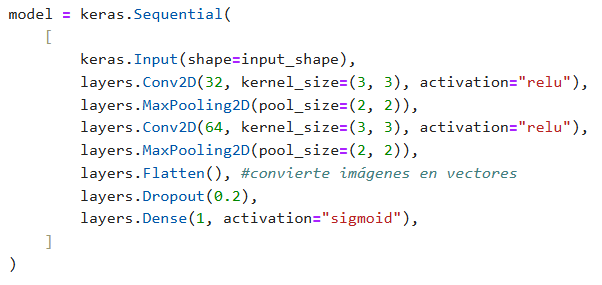
\includegraphics[width=0.99\textwidth]{img/cnn_propia.PNG}
    \caption{CNN propia. Fuente propia}
    \label{fig:cnn_propia}
\end{figure}


\subsubsection{CNN AlexNet}

La segunda CNN realizada está basada en la CNN AlexNet. AlexNet fue creada en 2012 por Alex Krizhevsky. Se trata de una red pre entrenada diseñada para reducir el error en la clasificación de imágenes para el proyecto ImageNet \cite{codificandobits24} (base de datos que proporciona una gran cantidad de imágenes etiquetadas para la IA \cite{datasmarts24}). Obtuvo muy buenos resultados de entrenamiento y supuso un gran avance en las arquitecturas de aprendizaje profundo \cite{diego23} aunque, al tratarse de una CNN muy profunda, requiere de un GPU (debido a su elevado coste computacional) y de una gran cantidad de datos para su correcto funcionamiento. 

Esta CNN está compuesta por cinco capas convolucionales. La primera, segunda y quinta capa convolucional están seguidas por una capa con la que se selecciona el máximo valor de un área (max-pooling) de 3×3 \cite{LMO24}. La primera capa convolucional incluye un filtro (\textit{kernal\_size})  de 11x11 y una reducción de dimensiones significativa (\textit{padding} = 4). En las siguientes capas convolucionales, el tamaño de filtro es menor (5×5 y 3×3) \cite{diego23}. Seguidamente, la CNN original de AlexNet contiene dos capas ocultas encargadas de la clasificación de las imágenes, de 4.096 neuronas cada una, y de una última capa densa de salida de 1.000 neuronas \cite{LMO24}. Figura \ref{fig:resumen_alexNet}. Pero, tanto las capas ocultas como la última capa densa han sido modificadas en este trabajo por tres modelos distintos con diferente número de capas ocultas.

\begin{figure}[h]
    \centering
    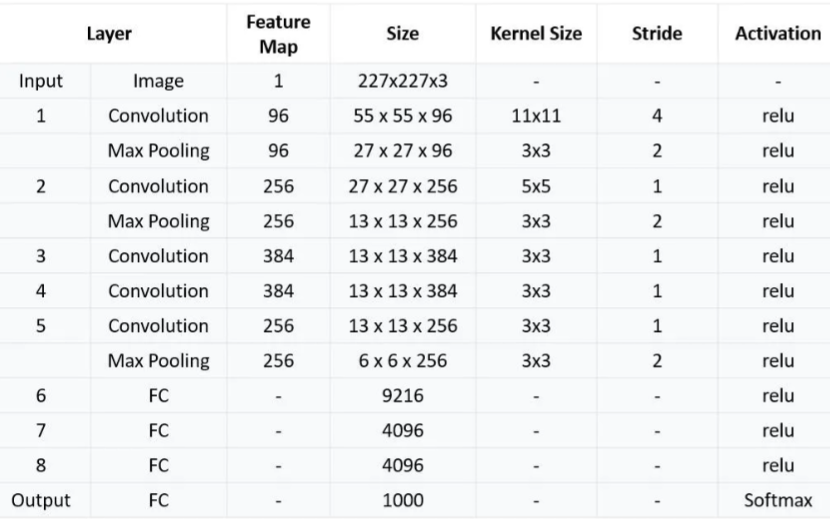
\includegraphics[width=0.99\textwidth]{img/resumen_alexNet.PNG}
    \caption{Resumen AlexNet. \cite{Medium24}}
    \label{fig:resumen_alexNet}
\end{figure}

\subsubsection{\textit{Batch size} y arquitectura}
En primer lugar, se han realizado dos tablas comparativas entre 3 arquitecturas de modelos diferentes y 4 valores de \textit{batch size} para la CNN propia y la CNN AlexNet.

La primera arquitectura se corresponde con un modelo que posee varias capas convolucionales (con las que se obtienen características importantes de las imágenes) seguidas de capas de MaxPooling2D para reducir la dimensionalidad. No posee capas ocultas. Finalmente se encuentra una capa densa de salida. 

De antemano ya se puede deducir que, este modelo es muy simple y, los resultados no van a ser buenos por lo que de descartará. Pero, así también se puede comprobar la mejora del modelo ajustándolo correctamente.

La segunda arquitectura se corresponde con un modelo que posee varias capas convolucionales (con las que se obtienen características importantes de las imágenes) seguidas de capas de MaxPooling2D para reducir la dimensionalidad. También hay una capa oculta de 100 neuronas y una capa densa de salida. 

La presencia de capas ocultas provoca una mejor capacidad para aprender de los datos del modelo ya que, al interconectarse la capa oculta con los datos de entrada, aprende características significativas de las características de entrada.

Por último, la tercera arquitectura, se corresponde con un modelo que posee varias capas convolucionales (con las que se obtienen características importantes de las imágenes) seguidas de capas de MaxPooling2D para reducir la dimensionalidad. En este caso, existen dos capas ocultas con 100 neuronas en la primera capa, y 16 neuronas en la segunda capa y, una capa densa de salida.

A su vez, se han probado 4 valores distintos (todos ellos potencias de 2) de \textit{batch size} para identificar el mejor modelo y el valor de \textit{batch size} con el que funciona mejor este modelo tanto con la CNN propia como con la CNN AlexNet.

Tal y como ya se ha comentado en los conceptos teóricos, el \textit{batch size} tiene un impacto importante en la precisión, velocidad y estabilidad del modelo y, dependiendo del objetivo puede funcionar mejor un \textit{batch size} u otro. Por eso, se busca determinar cuál es el ideal en este caso.

\subsubsection{Número de neuronas}
Una vez elegida la mejor CNN, el mejor modelo acorde a la arquitectura y el \textit{batch size}, se compara este modelo para distintos valores de neuronas en la capa oculta (todos estos valores son potencia de 2).

A mayor número de neuronas en la capa oculta, mejor se va a comportar la red con los datos de entrenamiento dado que, la capacidad de memorización de la red es mayor. Pero, peor se va a comportar con los datos de validación o prueba ya que no los ha visto ~\cite{diego23}. Por ello, es importante probar distintos valores y determinar cuál es el mejor para este caso.






\capitulo{5}{Resultados}

\section{Resumen de resultados}

Como ya se ha comentado previamente en los apartados de ``Objetivos'' y ``Metodología'', en este trabajo se han realizado diversas comparaciones con el fin de encontrar el mejor modelo de red neuronal acorde a nuestro caso, es decir, para determinar correctamente si existe o no neumonía a partir de un conjunto de imágenes médicas de CXT.

Hay que tener en cuenta que, cada vez que se ejecuta el código de Python realizado para la obtención de predicciones de imágenes a partir de redes neuronales, los resultados pueden variar sutilmente debido principalmente a:
\begin{itemize}
    \item El valor de los pesos iniciales (w) se asignan de manera aleatoria. Por lo que, cada vez que se ejecuta el entrenamiento, los pesos iniciales pueden ser distintos, lo que lleva a resultados ligeramente diferentes en las predicciones.
    \item Las muestras de entrenamiento también se seleccionan de manera aleatoria por lo que, en cada ejecución el subconjunto de datos seleccionado para entrenar el modelo puede ser distinto, lo que hace variar ligeramente los resultados.
\end{itemize}

Por lo tanto, en cada ejecucion se parte de un estado diferente.

\subsection{Comparación entre arquitecturas y \textit{batch size} con CNN propia y CNN AlexNet}

En primer lugar, se ha realizado con Python una tabla comparativa entre tres modelos de arquitectura distintos (explicados en el apartado de ``Metodología'') y cuatro valores distintos de \textit{batch size} (8, 16, 20, 32, 64) tanto para la CNN propia como para la CNN AlexNet.

En dichas tablas, se han calculado diversas métricas para determinar cuál es el mejor modelo. Antes de comenzar a calcular las métricas, es necesario obtener la matriz de confusión para obtener los verdaderos positivos (TP), verdaderos negativos (TN), falsos positivos (FP) y falsos negativos (FN) y, a partir de estos valores se calculan las métricas.

\begin{figure}[h]
    \centering
    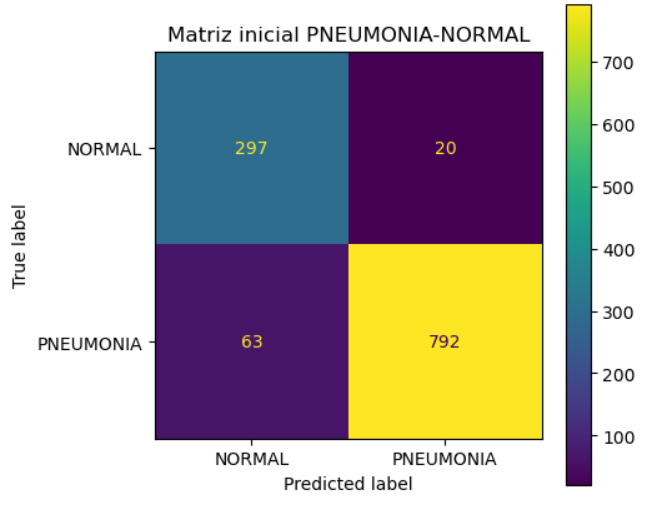
\includegraphics[width=0.80\textwidth]{img/matriz_conf_inicial.PNG}
    \caption{Matriz de confusión inicial. Fuente propia}
    \label{fig:matriz_confusion_inicial}
\end{figure}

\begin{itemize} 
    \item \textbf{Verdaderos positivos (TP)}: cantidad de positivos que fueron clasificados correctamente por el modelo como positivos. En la figura \ref{fig:matriz_confusion_inicial} se corresponde con los casos que el modelo predice como neumonía y realmente el paciente tiene neumonía (valor 792).
    \item \textbf{Verdaderos negativos (TN)}: cantidad de negativos que fueron clasificados correctamente por el modelo como negativos. En la figura \ref{fig:matriz_confusion_inicial} se corresponde con los casos que el modelo predice como normal y realmente el paciente no tiene neumonía (valor 297).
    \item \textbf{Falsos positivos (FP)}: cantidad de negativos que fueron clasificados incorrectamente por el modelo como positivos. En la figura \ref{fig:matriz_confusion_inicial} se corresponde con los casos que el modelo predice como neumonía pero realmente el paciente no tiene neumonía (valor 20).
    \item \textbf{Falsos negativos (FN)}: cantidad de positivos que fueron clasificados incorrectamente por el modelo como negativos. En la figura \ref{fig:matriz_confusion_inicial} se corresponde con los casos que el modelo predice como normal pero realmente el paciente tiene neumonía (valor 63).
\end{itemize}

Una vez obtenidos los TP, TN, FP y FN, se calculan las siguientes métricas:

\begin{itemize}
    \item \textbf{\textit{Loss}}: se emplea para evaluar cómo un modelo de aprendizaje automático se ajusta a los datos de entrenamiento.
    
    Para calcular el valor de \textit{loss} en Python, no se emplea una fórmula concreta dada su complejidad sino que, se calcula mediante la función \textit{model.evaluate} que proporciona la biblioteca keras.
    \item \textbf{\textit{Acuracy} (o exactitud)}: proporción de predicciones correctas. 
    \begin{equation*}
        \text{\textit{accuracy}} = \frac{\text{TP + TN}}{\text{TN + FP + FN + TP}}
    \end{equation*}
    \item \textbf{\textit{Precision}}: proporción de predicciones positivas correctas
    \begin{equation*}
        \text{\textit{precision}} = \frac{\text{TP}}{\text{TP + FP}}
    \end{equation*}
    \item \textbf{\textit{Recall} (o sensibilidad)}: proporción de positivos detectados
    \begin{equation*}
        \text{\textit{recall}} = \frac{\text{TP}}{\text{TP + FN}}
    \end{equation*}
    \item \textbf{F1}:  media armónica de precisión y exhaustividad para evaluar de una forma más equilibrada el rendimiento del modelo.
    \begin{equation*}
        \text{F1} = \frac{\text{2 * \textit{precision} * \textit{recall})}}{\text{\textit{precision}+\textit{recall}}}
    \end{equation*}
    \item \textbf{\textit{Specificity} (o especificidad)}: proporción de negativos detectados
    \begin{equation*}
        \text{\textit{specificity}} = \frac{\text{TN}}{\text{TN + FP}}
    \end{equation*}
    \item \textbf{fpr (o tasa de falsos positivos)}: proporción de negativos incorrectamente clasificadas como positivos, respecto al total de casos negativos reales.
    \begin{equation*}
        \text{fpr} = \frac{\text{FP}}{\text{FP + TN}}
    \end{equation*}
    \item \textbf{fnr (o tasa de falsos negativos)}: proporción de positivos incorrectamente clasificadas como negativos, respecto al total de casos positivos reales.
    \begin{equation*}
        \text{fnr} = \frac{\text{FN}}{\text{FN + TP}}
    \end{equation*}
    \item \textbf{AUC (o área bajo la curva ROC)}: se emplea para evaluar la capacidad de distinción entre clases positivas y negativas de un modelo de clasificación binaria. Un 1 significa que es capaz de distinguir perfectamente entre clases, un 0.5 significa una clasificación aleatoria y un 0 indica que ninguna clase ha sido correctamente clasificada. Esto se puede ver mejor en la figura \ref{fig:roc}.
    \begin{figure}[h]
        \centering
        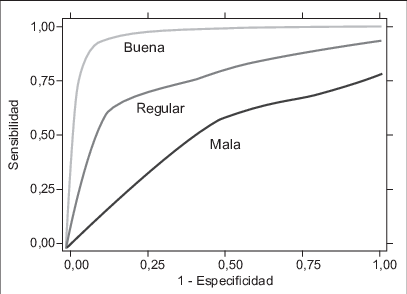
\includegraphics[width=0.70\textwidth]{img/roc.png}
        \caption{Ilustración tipos de curvas ROC. ~\cite{ResearchGate24}}
        \label{fig:roc}
    \end{figure}
    
    Para calcular el valor de AUC en Python, no se emplea una fórmula concreta dada su complejidad, sino que, se calcula mediante la función \textit{roc\_auc\_score} del módulo sklearn.
    
\end{itemize}

Una vez se han obtenido todos estos parámetros para cada una de las arquitecturas y cada uno de los valores de \textit{batch size} se comparan y se determina, cuál de las dos CNN funciona mejor y, una vez se tiene esto, se decide cual es la mejor arquitectura y, para esa arquitectura concreta se determina cual es el mejor valor de \textit{batch size}. Hay que tener en cuenta que, la mejor arquitectura es aquella con un valor mayor en todas las métricas (excepto \textit{loss}, fpr y fnr que interesa un valor menor).

\begin{figure}[h]
    \centering
    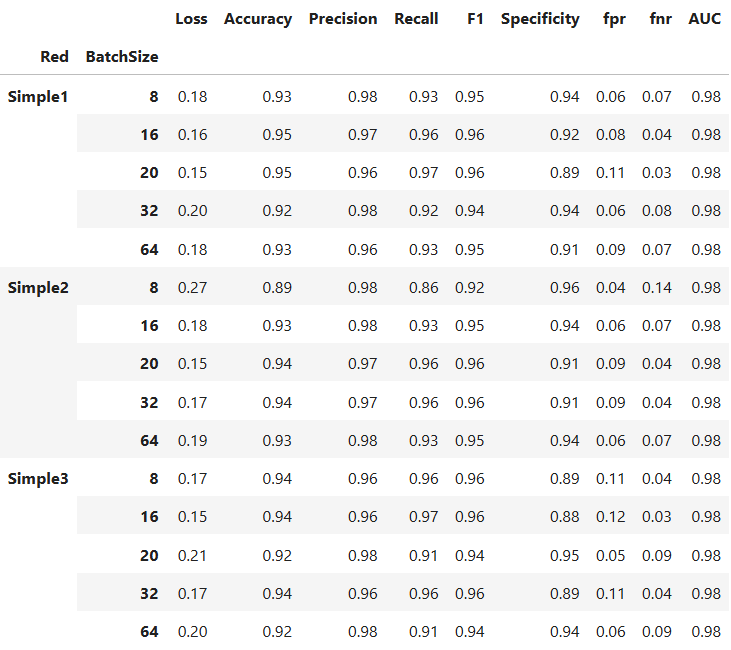
\includegraphics[width=0.99\textwidth]{img/tabla_propia_arqu_batch.PNG}
    \caption{Tabla comparativa de las distintas arquitecturas y \textit{batch size} con CNN propia. Fuente propia.}
    \label{fig:tabla_propia_arqu_batch}
\end{figure}
\FloatBarrier


\begin{figure}[h]
    \centering
    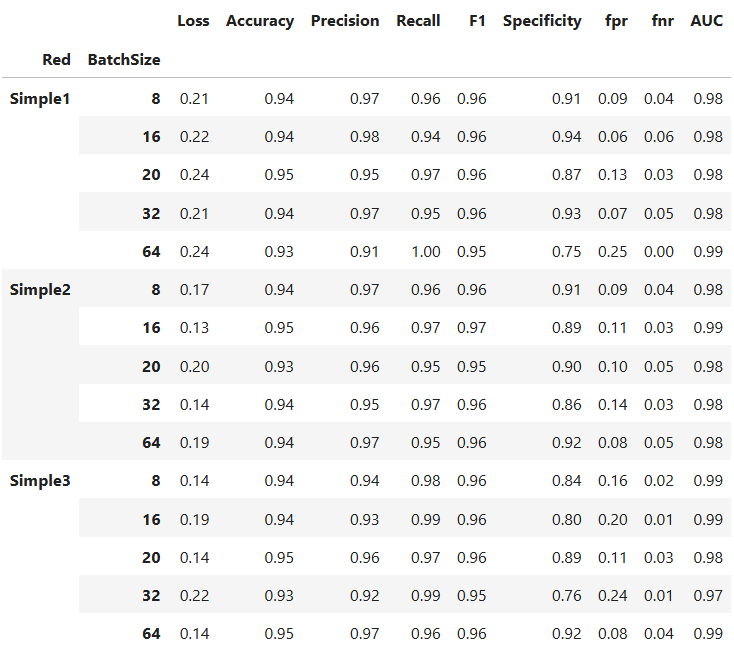
\includegraphics[width=0.99\textwidth]{img/tabla_alexNet_arqu_batch.PNG}
    \caption{Tabla comparativa de las distintas arquitecturas y \textit{batch size} con CNN AlexNet. Fuente propia.}
    \label{fig:tabla_alexNet_arqu_batch}
\end{figure}
\FloatBarrier

Previo a dictaminar los mejores resultados obtenidos en este caso, hay que tener en cuenta la aleatoriedad de pesos y muestras iniciales mencionados previamente, por lo que se obtienen resultados ligeramente distintos en cada ejecución. Debido a esto y a la similitud en los resultados obtenidos, se ha comprobado como cada vez que se ejecutaba se obtenían los mejores resultados en un modelo o en otro (excluyendo el modelo ``Simple1'' debido a su simplicidad). Por lo que, a continuación, se va a determinar el mejor modelo obtenido en este caso (en la ejecución del \textit{notebook} ``redes neuronales - neumonia'').

En primer lugar, con las tablas obtenidas para la CNN propia \ref{fig:tabla_propia_arqu_batch} y la de AlexNet \ref{fig:tabla_alexNet_arqu_batch}, se puede observar como en la tabla referida a la CNN de AlexNet existen valores mayores de AUC (una métrica que puede resultar muy interesante en este caso debido al desbalanceo que existe entre casos y controles) ya que hay varios valores de 0,99 mientras que en la de CNN propia en ningún caso sube de 0,98. Por lo tanto, se puede descartar la CNN propia y, a partir de ahora se trabaja con la CNN de AlexNet.

Antes de identificar la arquitectura óptima, hay que tener en cuenta que, el modelo ``Simple1'' es demasiado básico. En consecuencia, los resultados que ofrece no son muy buenos ya que, carece de capas ocultas y su arquitectura es extremadamente simple. Por lo que ha sido la primera arquitectura en descartarse. Sin embargo, es de gran utilidad para comprobar lo mal que predice el modelo en un principio y como este evoluciona. 

Ya que, tal y como se muestra en la figura \ref{fig:matriz_confusion_inicial}, donde se visualiza la matriz de confusión del modelo más simple (``Simple1'') con la CNN propia, se observa como en el hipotético caso de que este modelo no se mejorara y fuera utilizado en la vida real, 63 pacientes con neumonía serían diagnosticados como normal y 20 pacientes sin neumonía serían diagnosticados con neumonía. Esto supone unas cifras demasiado altas y acarrearía graves consecuencias en el ámbito de la sanidad. Por ello es necesario mejorar este modelo.

Una vez descartada la primera arquitectura, se realiza una comparación entre la segunda (``Simple2'') y la tercera (``Simple3''). Observando la \ref{fig:tabla_alexNet_arqu_batch} se puede determinar que, aunque los resultados son similares para ambas arquitecturas, existen valores mayores de AUC en el modelo ``Simple3'' y, por ellos se escoge como la mejor arquitectura. Como ya se ha comentado en el apartado de ``Metodología'', el modelo "Simple3" se corresponde con un modelo que posee varias capas convolucionales (con las que se obtienen características importantes de las imágenes) seguidas de capas de MaxPooling2D para reducir la dimensionalidad. También hay una capa oculta de 100 neuronas, una segunda capa oculta de 16 neuronas y una capa densa.

Una vez escogida la arquitectura, se determina cual es el mejor \textit{batch size} para esta arquitectura. De nuevo, observando la tabla \ref{fig:tabla_alexNet_arqu_batch}, se puede ver como los valores más altos de AUC existen para un \textit{batch size} de 8, 16 y 64 y, teniendo en cuenta que un \textit{batch size} mayor entrena la red en menos tiempo ya que, el \textit{batch size} es un compromiso entre precisión y tiempo de entrenamiento, el mejor \textit{batch size} en este caso es el de 64.

Resumiendo, se puede determinar que, en esta primera comparación y con lo que se va a trabajar a partir de ahora es la \textbf{CNN de AlexNet}, el modelo \textbf{``Simple3''} con un \textbf{\textit{batch size} de 64}.

\subsection{Comparación número de neuronas}
Partiendo de la CNN de AlexNet con el modelo ``Simple3'' y un \textit{batch size} de 64, se comparan distintos valores de neuronas en la capa oculta para este modelo.

El modelo ``Simple3'' presenta dos capas ocultas con neuronas. En este caso, para probar los distintos valores de neuronas en las capas ocultas, se han empleado los mismos valores en ambas capas, aunque, también se podría haber hecho diferenciando valores entre una capa y otra. Por lo general, la primera capa tiene el mismo o más neuronas que la segunda, y así sucesivamente. Los valores empleados han sido potencias de 2 tales como 512, 1024 y 2048.

Se emplean las mismas métricas que en el caso anterior para decidir cuál es el mejor modelo. Lo ideal es que todas las métricas excepto ``\textit{loss}'', ``fpr'' y ``fnr'' tengan el mayor valor. 

\begin{figure}[h]
    \centering
    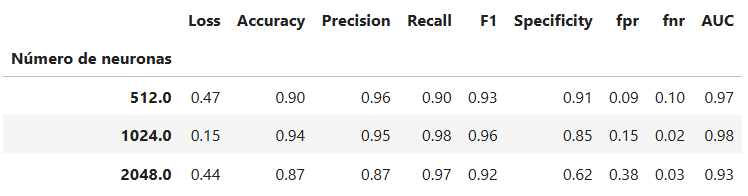
\includegraphics[width=0.99\textwidth]{img/tabla_num_neuronas.PNG}
    \caption{Tabla comparativa de distintos valores de neuronas en la capa oculta. Fuente propia.}
    \label{fig:tabla_num_neuronas}
\end{figure}
\FloatBarrier

Tal y como se puede observar en la tabla \ref{fig:tabla_num_neuronas}, comparando cada una de las métricas para los tres valores diferentes se puede ver que los resultados de las métricas son similares pero, fijándonos en el AUC, el mejor valor se encuentra para 1024 neuronas.

Aun así, comparando las métricas obtenidas para 1024 neuronas en las dos capas ocultas en comparación con las métricas de la tabla \ref{fig:tabla_alexNet_arqu_batch} en el modelo ``Simple3'', con un \textit{batch size} de 64 y 100 y 16 neuronas respectivamente en ambas capas ocultas (que son los valores que se han empleado en el modelo inicial) se puede concluir que, el mejor modelo se corresponde con la CNN de AlexNet, el modelo ``Simple3'', un \textit{batch size} de 64, y 100 y 16 neuronas en las capas ocultas respectivamente.

Con este modelo final se obtiene un AUC del 99\%, un \textit{accuracy} del 95\%, y una precisión del 97\% tal y como se puede observar en la figura \ref{fig:tabla_alexNet_arqu_batch}.

Para el modelo elegido finalmente, se ha obtenido tanto su matriz de confusión \ref{fig:matriz_conf_final} (para ser comparada con la matriz inicial \ref{fig:matriz_confusion_inicial}) como dos gráficas donde se representa el rendimiento del modelo a lo largo de tiempo en el entrenamiento y la validación respecto al AUC \ref{fig:grafica_auc_Simple3_64_100_16} y respecto a \textit{loss} \ref{fig:grafica_loss_Simple3_64_100_16}.  

\begin{figure}[h]
    \centering
    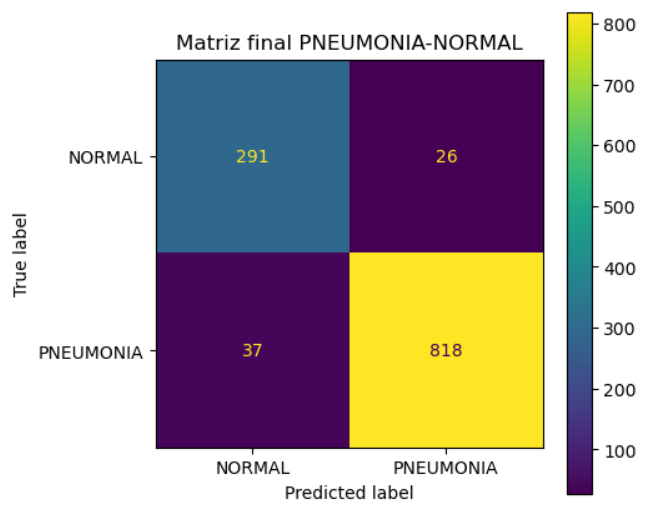
\includegraphics[width=0.80\textwidth]{img/matriz_conf_final.PNG}
    \caption{Matriz de confusión modelo final. Fuente propia.}
    \label{fig:matriz_conf_final}
\end{figure}

Con la matriz de confusión final \ref{fig:matriz_conf_final}, se puede apreciar cómo el valor de FP aumenta mientras que los FN disminuyen notablemente respecto a la matriz inicial. 

Tal y como se ha comentado al principio de este apartado, los FP se corresponden con aquellos pacientes sin neumonía diagnosticados por el modelo con neumonía y, los FN son aquellos que el modelo identifica como normal (o sano) pero en verdad se trata de un paciente con neumonía.

En el ámbito clínico, es preferible un modelo con un mayor número de FP que de FN ya que, los FP serán revisados más exhaustivamente por el personal clínico, quienes acabarán viendo que el paciente no tiene dicha enfermedad, por lo que no resulta en algo muy perjudicial para el paciente. Sin embargo, los FN, pueden ser mucho más peligrosos ya que, se diagnostica a un paciente como sano estando enfermo, lo que puede agravar la patología al no diagnosticarse a tiempo y causar daños irreparables para el paciente.

Por lo tanto, teniendo en cuenta esto último y comparando la matriz de confusión inicial \ref{fig:matriz_confusion_inicial} con la matriz de confusión final, \ref{fig:matriz_conf_final} se puede apreciar una mejora considerable ya que, aunque en la matriz de confusión final el valor de FP aumente, esto no es un problema serio en este caso. Además, el valor de FN disminuye notablemente, algo muy positivo a tener en cuenta debido a las consecuencias que esto puede acarrear.


\begin{figure}[h]
    \centering
    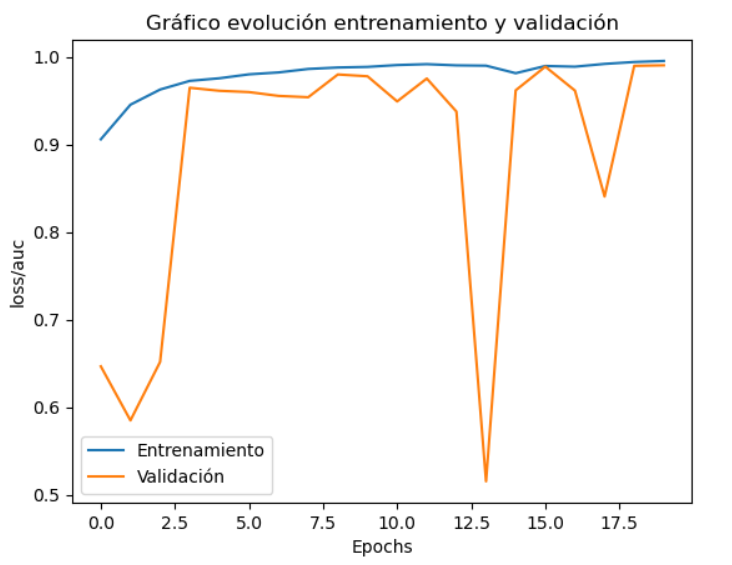
\includegraphics[width=0.80\textwidth]{img/grafica_auc_Simple3_64_100_16.PNG}
    \caption{Gráfica AUC rendimiento del entrenamiento y la validación del modelo final. Fuente propia.}
    \label{fig:grafica_auc_Simple3_64_100_16}
\end{figure}
\FloatBarrier

En la gráfica \ref{fig:grafica_auc_Simple3_64_100_16}, se visualiza el rendimiento del modelo final (``Simple3'' \textit{batch size} = 64 y 100 y 16 neuronas en las últimas capas) respecto a la métrica ``AUC'' a lo largo de tiempo tanto para el entrenamiento como la validación. Este tipo de gráficas sirven para determinar si el modelo está aprendiendo correctamente o, por el contrario, existe sobreajuste o subajuste.

Los valores de AUC obtenidos durante el entrenamiento (``auc''), miden la capacidad del modelo para distinguir entre clases en el conjunto de entrenamiento mientras que los valores de AUC obtenidos durante la validación (``val\_auc'') miden la capacidad del modelo para distinguir entre clases en el conjunto de validación. En ambos casos, un valor mayor indica un mejor modelo.

Por lo tanto, tal y como se puede apreciar en la gráfica \ref{fig:grafica_auc_Simple3_64_100_16} la línea de entrenamiento comienza en las primeras épocas con un AUC de 0,9 aproximadamente y, a medida que pasan las épocas, el AUC aumenta casi hasta 1, lo que significa que el modelo mejora su capacidad para clasificar correctamente los ejemplos en el conjunto de entrenamiento a medida que las épocas avanzan. Así mismo, la línea de validación presenta dos picos notables en la época 2 y la época 13 (aproximadamente) y un pico algo menor en la época 17 donde el AUC es menor. Esto puede deberse a un sobreajuste temporal o a unos datos empleados para la validación en esas épocas especialmente atípicos (diferentes al resto), lo que dificulta su identificación.

\begin{figure}[h]
    \centering
    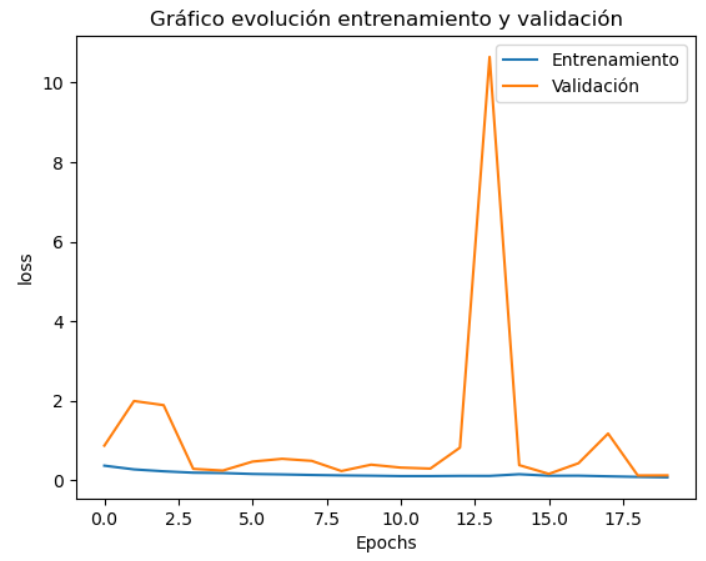
\includegraphics[width=0.80\textwidth]{img/grafica_loss_Simple3_64_100_16.PNG}
    \caption{Gráfica ``\textit{loss}'' rendimiento del entrenamiento y la validación del modelo final. Fuente propia.}
    \label{fig:grafica_loss_Simple3_64_100_16}
\end{figure}
\FloatBarrier

Por otro lado, en la gráfica \ref{fig:grafica_loss_Simple3_64_100_16}, se visualiza el rendimiento del modelo final respecto a la métrica ``\textit{loss}'' a lo largo de tiempo tanto para el entrenamiento como la validación. 

Los valores de \textit{loss} obtenidos durante el entrenamiento (``\textit{loss}''),miden el error del modelo en el conjunto de entrenamiento mientras que los valores de \textit{loss} obtenidos durante la validación (``val\_loss'') miden el error del modelo en el conjunto de validación. En ambos casos, un valor lo más cercano al 0 indica un mejor modelo.

Por lo tanto, tal y como se puede apreciar en la gráfica \ref{fig:grafica_loss_Simple3_64_100_16} la línea de entrenamiento comienza en las primeras épocas con un error (``\textit{loss}'') de 0,4 aproximadamente y, a medida que pasan las épocas, el error va disminuyendo acercándose al 0, lo que significa que el modelo está aprendiendo correctamente en el conjunto de entrenamiento. Así mismo, la línea de validación presenta un gran pico en la época 13 y dos picos menores en la época 2 y la época 17 (aproximadamente) donde el error es mayor. Esto puede deberse, de igual manera que ocurría en la gráfica referida al AUC, a un sobreajuste temporal o a unos datos empleados para la validación en esas épocas especialmente atípicos (diferentes al resto) lo que dificulta su identificación.

\section{Discusión.}

En primer lugar, hay que tener en cuenta que se trata de unos resultados obtenidos a partir de un CPU convencional en un ordenador personal. Ya que, debido a diversos problemas explicados en la sección de ``Inconvenientes'' del siguiente apartado, no se ha podido acceder a ningún supercomputador. 

Por lo tanto, estos resultados presentan algunas limitaciones. El ordenador personal no posee la misma capacidad de procesamiento y memoria que los supercomputadores por lo que, se ha tenido que reducir el número de épocas durante el entrenamiento lo que provoca unos resultados subóptimos afectando en su precisión y eficacia.

Teniendo en cuenta esto y que los resultados obtenidos no son los ideales, se trata de unos resultados razonablemente buenos ya que, tal y como se puede ver en la tabla \ref{fig:tabla_alexNet_arqu_batch} se ha alcanzado un AUC de 0,99, un error de 0,14, una exactitud de 0,95 y una precisión de 0,97. Además, en las gráficas obtenidas se puede ver cómo, a pesar de tener tres picos donde el conjunto de entrenamiento no se generalizan correctamente con el conjunto de validación, no se trata un comportamiento mantenido a lo largo de todas las épocas ya que, el modelo se corrige en las épocas posteriores.

Los tres picos obtenidos en las gráficas \ref{fig:grafica_loss_Simple3_64_100_16} y \ref{fig:grafica_auc_Simple3_64_100_16}, también pueden deberse a una poca cantidad de datos para el entrenamiento de una red neuronal ya que, otro punto a tener en cuenta es que, para un correcto entrenamiento de una red neuronal convolucional es necesario emplear grandes cantidades de datos \cite{kundu2021pneumonia} y, en este caso aun tratándose de un gran número de imágenes (5856 concretamente), en el ámbito de redes neuronales son necesarias muchas más para trabajar de forma idónea. Mas aun, teniendo en cuenta que se emplea la CNN de AlexNet donde cuanto más grande y variado sea el conjunto de datos, mejor rendimiento y generalización se obtiene del modelo.

En la matriz de confusión se observa un gran número de casos donde el modelo predice correctamente tanto los casos de neumonía (valor 818) como los casos sin ella (valor 291) y, 37 casos han sido diagnosticados como normal siendo neumonía, un valor mucho menor que el inicial.

Para concluir, se han obtenido resultados relativamente buenos teniendo en cuenta todos estos problemas, pero, aún queda mucho trabajo por hacer antes de poder introducir este tipo de IA en el ámbito clínico. Ya que, para eso es necesario contar con resultados prácticamente perfectos en todos los sentidos y, por ahora no es el caso.






\capitulo{6}{Conclusiones}

\section{Aspectos relevantes.}

Finalmente, se puede concluir que, se ha cumplido en mayor o menor medida con todos los objetivos estipulados en este trabajo:
\begin{itemize}
    \item Para comparar todos y cada uno de los resultados mencionados a continuación, se ha desarrollado una función para calcular una serie de métricas con las que se comparan los distintos modelos.
    \item Se han desarrollado dos CNN distintas, una propia y otra obtenida a partir de la CNN AlexNet, se han comparado y se ha determinado que, para este caso concreto, funciona mejor la CNN AlexNet.
    \item Se han desarrollado tres modelos de arquitectura diferentes, cada uno de ellos con distinto número de capas ocultas y, se ha determinado con cuál de los tres se obtienen mejores resultados de las métricas. Los modelos ``Simple2'' y ``Simple3'' estaban bastante a la par, aunque, en la prueba concreta realizada, los mejores resultados se han obtenido para el modelo ``Simple3'' (con dos capas ocultas).
    \item Se han modificado algunos hiperparámetros, se han comparado los resultados obtenidos con distintos \textit{batch size} y se ha determinado que el \textit{batch size} de 64 es el que funciona mejor para el modelo ``Simple3''.
    \item Se ha comprobado que, aumentando el número de neuronas en las capas ocultas del modelo Simple3, no se obtienen mejores resultados por lo que, se han mantenido los valores iniciales de neuronas (100 y 16 respectivamente).
    \item Para el desarrollo de este trabajo, se ha empleado la herramienta keras para la creación de redes neuronales profundas en Python. Esto supone un aprendizaje que puede resultar muy útil de cara al futuro ya que keras es una herramienta muy popular en IA.
    \item Gracias a los numerosos artículos leídos acerca de la neumonía y las CXT, se ha podido profundizar mucho más acerca de esta patología y su método diagnóstico. También se ha aprendido mucho acerca de las imágenes médicas y la forma de identificar la patología. 
    
\end{itemize}

También hay que mencionar que, al no haber podido acceder a ningún supercomputador y haber trabajado a nivel de CPU con el ordenador personal, se ha tardado mucho más en ejecutar las funciones, lo que ha retrasado el trabajo y, también, se han tenido que disminuir el número de épocas a ejecutar por lo que, los resultados obtenidos no son los óptimos.

Como conclusión final, se puede afirmar que, con este trabajo se han adquirido grandes conocimientos en el ámbito de IA y redes neuronales profundas, además de en lo referente a neumonía y CXT, lo que puede ser de gran ayuda para un futuro en el ámbito de la Ingeniería de la Salud.

\subsection{Inconvenientes}

A la hora de realizar este trabajo, han surgido diversos inconvenientes, desde cambios en los objetivos del TFG hasta problemas para acceder a más de un supercomputador.

En primer lugar, tal y como se explica en el \textit{Anexo A}, ha habido varios cambios hasta llegar al TFG definitivo. Resumiendo lo indicado en este Anexo, se cambió de TFG hasta en tres ocasiones debido a diferentes problemas. El primer TFG consistía en la identificación de cáncer de pulmón a partir de imágenes de TAC entrenando una red neuronal. El problema de este TFG fue el tipo de imágenes con el que se iba a trabajar ya que, las imágenes de TAC son imágenes tridimensionales, lo que supone una gran complejidad a la hora de analizar cada uno de los cortes. En el segundo TFG, el objetivo era identificar cáncer de pulmón a partir de CXT anotando las imágenes y entrenando una red neuronal. Este TFG presentaba dos inconvenientes, el primero era la dificultad para conseguir que un médico especializado del hospital indicara en todas y cada una de las imágenes de CXT donde estaba exactamente el tumor y, el segundo problema fue la necesidad de ser aprobados por el comité de bioética para trabajar con las imágenes de CXT de pacientes del Hospital Universitario de Burgos (HUBU) ya que, tras la realización de un primer informe, este fue denegado y, ya no se llegaba a tiempo para una posible aprobación. Todos estos puntos están explicados con una mayor profundidad en el \textit{Anexo A}. Finalmente, la tercera opción de TFG sí ha podido realizarse, aunque, con otra serie de complicaciones mencionadas a continuación.

Ha habido varios problemas con GitHub y sus aplicaciones derivadas. En un principio, la idea era emplear ZenHub, una herramienta de gestión de proyectos que trabaja con GitHub para la planificación y seguimiento del proyecto, pero, había que pagar unos 10 euros mensuales por usuario ya que, el plazo para solicitar las plazas gratuitas para estudiantes se había acabado. Por lo que, se descartó esta opción. Después se barajaron otras opciones similares a ZenHub, como ``Asana'' o ``Jira'' pero, tras investigar más a fondo cada una de ellas se llegó a la conclusión de que solo ofrecían un mes de prueba y luego también había que pagar una mensualidad para su uso completo. Por lo que, finalmente se empleó únicamente GitHub para la planificación del trabajo.

Durante la realización del segundo TFG también surgieron otra serie de problemas ya que, a la hora de seguir los pasos indicados en el video \footnote{\url{https://www.youtube.com/watch?v=IOI0o3Cxv9Q}}, necesario para la realización de esta propuesta de TFG, se tuvo que instalar y desinstalar en numerosas ocasiones tanto la aplicación de Python como el entorno de anaconda empleado para el TFG debido a que las versiones necesarias para realizar lo indicado en el video tenían que ser muy concretas y causaban problemas con mucha facilidad.

Por último, también han surgido problemas a la hora de intentar acceder a un supercomputador. Primero se intentó acceder al Supercomputación de Castilla y León (SCAYLE) pero, tras enviar la solicitud y no recibir respuesta, se descubrió que, el supercomputador había dejado de funcionar durante los meses en los que estaba previsto su uso. Una vez se supo esto, se solicitó acceso al cluster de León para usar GPUs que tiene el cluster pero, tampoco se ha podido usar debido a una mala gestión en la asignación de recursos por parte de los administradores. Ya que, supuestamente tienen reservados unos 100 terabytes para ser usados por personas de Burgos con acceso a este cluster pero, estaba dando problemas empleando una capacidad mucho menor. Por lo que, a pesar de que se está trabajando para corregir este problema, no se llegaba a tiempo para poder usarlo en este trabajo. 

Finalmente, se ha trabajado con el ordenador personal a nivel de CPU. Esto ha supuesto que, los resultados obtenidos sean peores que si se hubiera empleado un supercomputador debido a las limitaciones de precisión y eficiencia, tal y como se ha comentado en el apartado de ``Resultados''.









\capitulo{7}{Lineas de trabajo futuras}

En este capítulo, se proponen diversas líneas de trabajo para continuar y mejorar el trabajo realizado.

\begin{itemize}
    \item Una línea futura para este trabajo consiste en realizar la anotación de cada una de las imágenes de radiografías de tórax con la ayuda de un médico especializado. De forma que, el profesional señale de forma precisa la ubicación de la neumonía y, así, la red neuronal puede entrenar las imágenes de una forma más precisa. Esta metodología, que se consideró inicialmente como una opción para este proyecto (en la segunda opción de TFG), no pudo llevarse a cabo en esta ocasión, pero puede tratarse de una gran mejora para futuros desarrollos.
    \item Otra línea futura puede ser, mejorar la red neuronal entrenada de forma que, no solo identifique la presencia de neumonía, sino que también, sea capaz de distinguir entre neumonía viral y bacteriana. Esta mejora, permitiría personalizar el tratamiento desde el primer momento, optimizando la atención médica y mejorando los resultados clínicos de los pacientes. Las imágenes con las que se trabaja en las carpetas de ``PNEUMONIA'' ya están calificadas como ``viral'' o ``bacteriana'' lo que simplifica el proceso.
    \item Una visión a futuro más lejano, pero con una gran relevancia, es la aplicación de estas técnicas en el ámbito clínico para determinar tanto la presencia de neumonía como su localización exacta en una CXT. De forma que, cuando un paciente acuda a consulta y se le realice una CXT, el sistema proporcione de forma automática al médico, información precisa sobre la existencia (o ausencia) y localización de la neumonía. Esta implementación optimizaría el diagnóstico y tratamiento y mejoraría la atención al paciente a nivel mundial.
    \item En este caso, se trabaja con imágenes de radiografías de tórax de pacientes de entre 1 y 5 años por lo que, a la hora de analizar las imágenes, esta red neuronal está limitada a un rango de edad especifico. En un futuro, lo ideal sería añadir más imágenes, entre ellas imágenes de adultos a este entrenamiento para poder analizar la existencia de neumonía sin importar la edad.
    \item Mostrar al médico a partir de la CXT información acerca de la anomalía encontrada, si se encuentra en el pulmón derecho o el izquierdo, tipo, tamaño, densidad, homogeneidad, etc. 
    \item Realizar otra red neuronal de forma similar a esta, pero, incluyendo imágenes de CXT desde otros puntos de vista (además de la vista frontal) para así, poder abordar los problemas asociados con los ``puntos ciegos'' que pueden surgir al utilizar únicamente imágenes frontales. Al incluir nuevas vistas (como la lateral u oblicua), se espera mejorar la precisión y la robustez del modelo.
\end{itemize}



\bibliographystyle{apalike}
\bibliography{bibliografia}

\end{document}
